\chapter{Methodology}

In this chapter we will go over the methods used to build and train our own pose estimation model.

\section{Fully Rendered Datasets}

\subsection{Motivations and Objective}

We find ourselves in the situation where we want to train a 6D pose estimation model on a set of objects that is not present in any available dataset. Therefore the first essential step to developing our model is the creation of our own datasets for training and evaluation.

These datasets consist of a collection of images containing the object we wish to track, with associated ground truths encoding the pose of the tracked object for each image. Collecting this data in the real world is tedious and difficult, considering both the number of samples required for deep learning, and that any errors or biases will strongly affect the perfomance of the trained model. 

One possible solution is to use rendering software, which can generate potentially infinite quantites of training images with associated, perfectly accurate ground truths. However, while a model trained on this data could function in simulation, we have no guarantee whether it would also function in real life. This is because a simulated sensor and simulated enviroment are unable to reproduce unmodeled physical effects and noise in the same way a real sensor would with a real environment. This issue, dubbed the "reality gap"\cite{domainRandomization2}, is recurring in any field which relies on simulations to supply data.

Domain Randomization\cite{domainRandomization} is one of the most utilised methods for solving this issue. Its principle states that introducing sufficient variability in the simulated domain will allow the model to generalise to the real world with no additional training. This allows us to entirely skip the laborious data collection step and instead rely on a 3D model of the object we wish to track, which is usually readily available and accurate.

Thus our objective is the creation of a fully rendered dataset for our network, and the evalutation of the performance of the network trained on this synthetic data in real life applications.

\subsection{Generation Methodology}
\label{ss:ScrewDataset}

To render the images for our dataset, we used the Unity Perception package\cite{unityPerception}, which integrates domain randomization features into its pipeline. Unity Perception works by simulating a scene, and then rendering each simulated frame from the perspective of a virtual camera. 

When setting up the simulation, we specify the number of iterations to simulate and the number of frames to render for each iteration. At the beginning of each iteration, we call a set of randomizer scripts. These set one of the domain variables for the iteration, such as the pose of an object or the colour of the light source, by extracting its value from a pre-defined probability distribution. The scene is then updated according to these variables, rendered, and the associated ground truth saved.

\begin{figure}
    \centering
    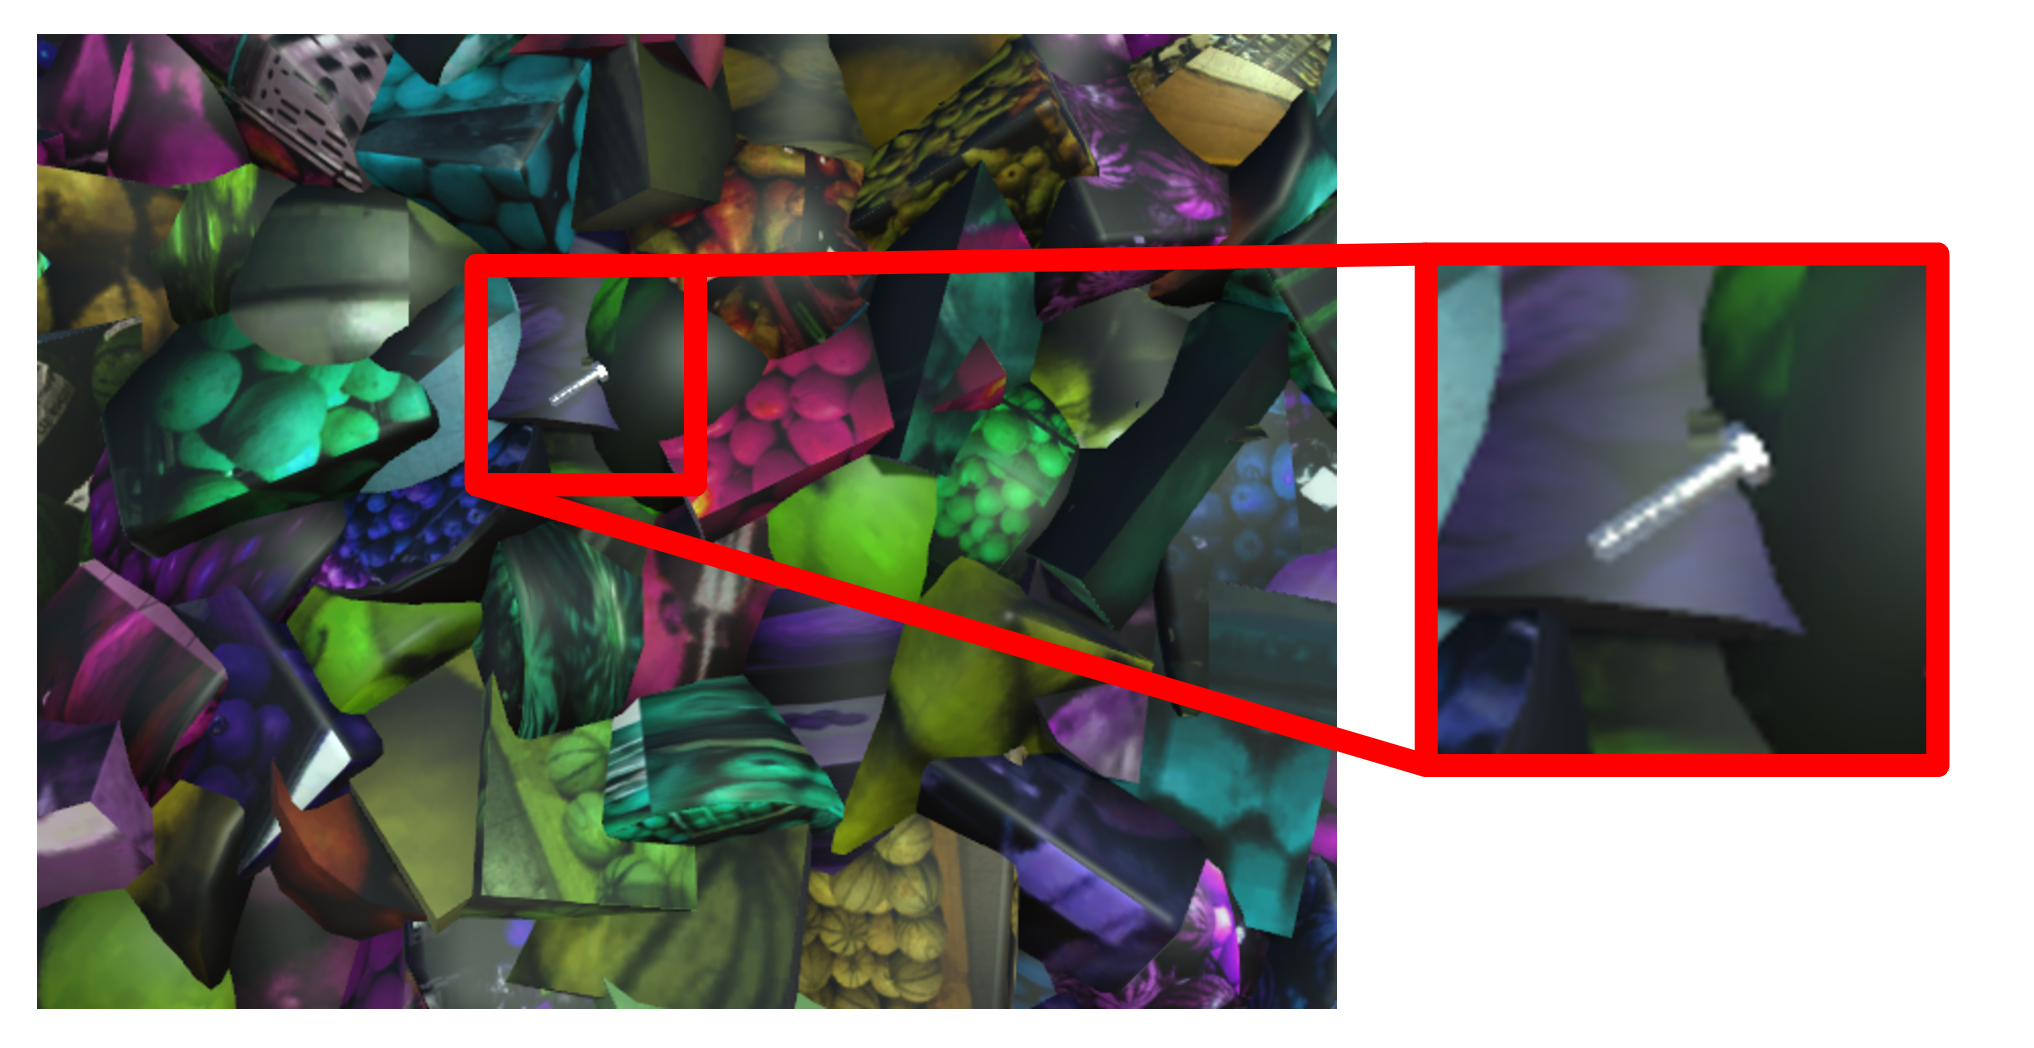
\includegraphics[width=0.6\textwidth]{screwdataset/ScrewDataset.png}
    \caption{One of the images generated with Unity's Perception package for training our model.}
    \label{fig:screwdataset}
\end{figure}

As a test case, we decided to generate a pose estimation dataset for a standard M6x30 hexagonal head screw. This is a very challenging object, as it is small and symmetric. Symmetric objects have always been difficult for pose estimation algorithms, due to reasons explained in depth in appendix 1. The model of the M6x30 screw was obtained from the FreeCAD Fasteners workbench\cite{Fasteners} and colored with a metallic texture.

The domain for this dataset consists of images of the screw placed inside of a scene: thus the primary domain variables are the pose, the background, and the lighting. We used a custom randomizer to set position and rotation for each iteration, and default randomizers provided as part of the Perception package to generate a background, composed by random 3D shapes placed with random positions, orientations and textures. Finally, we used a custom randomizer to set the lighting color, intensity and origin. A sample image from this dataset appears in figure \ref{fig:screwdataset}.

We can then interface the output of this procedure with EfficientPose using a conversion script, which performs the necessary tasks to make the dataset compatible with the generators used by the network. In this manner we can quickly and easily generate arbitrarily large datasets for training, by first running the Unity scenario, and then running the conversion script for EfficientPose.

\subsection{Training}

The original version of EfficientPose is trained on LINEMOD. However, the specifics of LINEMOD and of our own dataset are widely different: LINEMOD has around 1200 images per object, and only about 200 of these are used for training, while our dataset has 10000 images, 9000 of which are used for training. This means that we must set proper training parameters for our own dataset.

First, we reduced the number of epochs from 5000 to 100. Since our dataset contains 45 times more images, these two values represent a similar training time. EfficientPose also by default evaluates the model only every 10 epochs due to the small epoch size; we change this value to evaluate at the end of every epoch.

EfficientPose implements Keras' ReduceLRonPlateau callback to dynamically set the learning rate during training. This is standard practice: large learning rates quickly adjust the model but can lead to fluctuations, local minima and divergence; smaller learning rates avoid these issues but take an excessive amount of time to improve the model\cite{ReduceLR}. This method instead starts with a large learning rate, and then automatically reduces the learning rate whenever training stagnates, thus maintaining a value closer to the ideal. By default, EfficientPose halves the LR every time the accuracy does not improve for 25 epochs; we changed this to an 80\% reduction every 5 epochs, to account for the increased number of samples per epoch.

The initial and minimum learning rates are mantained identical to EfficientPose's, set at $10^{-4}$ and $10^{-7}$ respectively. For all purposes in this thesis, we will be using the networks scaled to their lowest hyperparameter $\phi = 0$, as going any higher requires inordinate amounts of time to train.

\subsection{Results}

\begin{figure}[ht]
    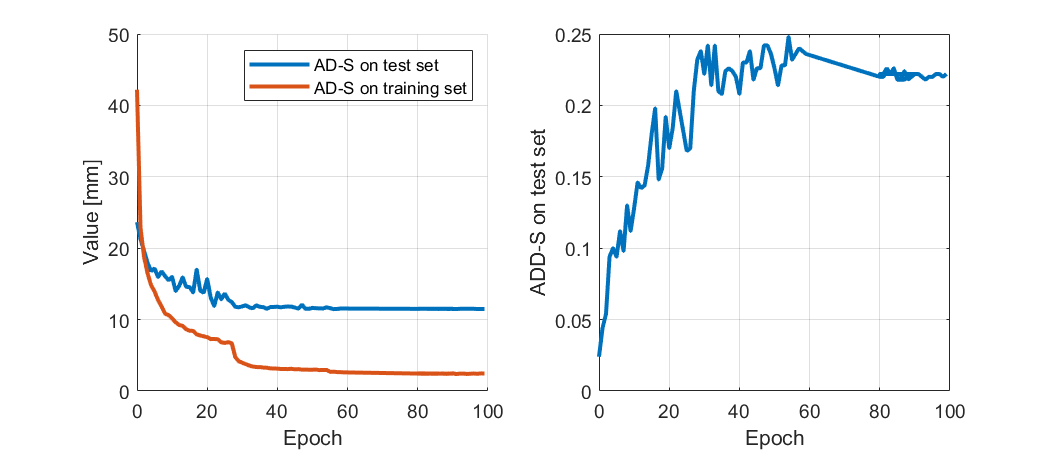
\includegraphics[width=\textwidth]{screwdataset_training.png}
    \caption{Evolution of the loss, AD-S and ADD-S metrics during training for the fully rendered dataset. The loss is computed as the AD-S metric on the training dataset.}
    \label{fig:screwdataset_training}
\end{figure}

After 100 epochs of training, the progress of which is shown in figure \ref{fig:screwdataset_training}, the model has a final ADD of 22.2\%, with a peak value obtained during training of 24.8\%, much lower than the 97.35\% reported by EfficientPose on LINEMOD. We can hypothesize that the reason for this performance gap is that the rendered dataset is much more difficult than LINEMOD, since we are dealing with a very small, symmetric object hidden inside a chaotic, colorful background with widely differing light conditions.

Another serious issue, that is more difficult to convey on paper, is that the model is not able to bridge the reality gap: while testing in real-life scenarios, it failed to identify the screw in most conditions, let alone produce accurate estimations. This means that it generalises poorly outside of the simulated environment, making it essentially unuseable in real applications.

\section{Augmented Reality Datasets}

\subsection{Motivations and Objective}

As stated above, the model trained on our custom dataset has very poor performance, both in simulated scenarios and in real-life applications. Since the same model has no similar issues when trained on LINEMOD, we can hypothesize that the cause lies with the training dataset itself, for two reasons:

\begin{enumerate}
    \item The training images are too difficult compared to the task we want to perform, preventing the network from learning properly.
    \item The training images and the real-life captures are excessively different, thus the model is not able to bridge the reality gap.
\end{enumerate}

The second issue is the most debilitating, as it makes whatever model we train completely unapplicable to any real life situation. We hypothesize that, since the backgrounds we generated are composed of a compact assortment of random shapes, with random sizes, colors, texures and poses, the resulting dataset is adeguate for representing extremely cluttered and noisy environments, but inadeguate for most other environments.

We have two options for facing this issue. The first would be to make the backgrounds more general in scope. This could mean, for example, generating a wider variety of synthetic backgrounds, or using sets of photographs, such as the COCO or Imagenet datasets \cite{DPOD}. This would allow the model to generalise to more situations, including eventually our usecase. This is probably the best option if we forsee a wide application of the model in a variety of different conditions, for example in an autonomous driving scenario.

The second option is to generate a set of training images that more accurately depict a small number of chosen environments. This makes it easier for the model to bridge the reality gap by making this gap "smaller", reducing the differences between the training dataset and the typical image seen during inferencing. However, we have fewer guarantees on performance outside of the selected environments, which makes this approach better for usecases which are stationary or limited to fewer settings. This is often the case for industrial applications, making this second option our preferred choice.

Thus our objective is to create a method to easily and quickly generate a realistic training dataset for our testing environment, which is a simple table with the objects placed on its surface. To do this, we will use an "Augmented Reality" approach, rendering the dataset objects on top of real images captured from the testing area.

\subsection{Generation Methodology}

We again use Unity Perception to generate our training dataset, as described in \ref{ss:ScrewDataset}. We used models for 5 objects: the same M6x30 screw used previously, a M8x16 round head screw, a M8x25 and M8x50 socket head screws, and a M4x40 countersunk screw. As previously stated, these are small, symmetric objects that are generally challenging to identify, with the additional complication that they all have similar shapes and sizes. Only the first four  are annotated, while the M4x40 is included as a "decoy" to reduce the number of false positives.

The key issue now becomes the positioning of the objects in the image. Since in real-life conditions, the pose of an item is almost always influenced to some degree by its environment, we believe that simply placing the item freely in 6D space as we did in the previous approach would lose information compared to a realistic placement. Taking our example setting where the objects are placed on a surface, this constrains three degrees of freedom for each object: the vertical position relative to the surface, and the two rotations around the axises that determine the surface itself. Thus our objective is, for each background image, to start from the pose of the surface relative to the camera, and from there generate a realistic pose for each dataset object, so that the object appears to be placed on the surface.

This pose is generated using the composition in sequence of three roto-translations:

\begin{enumerate}
    \item An initial transformation $(t_s, \text{R}_s)$ from the camera frame to the surface's reference frame.
    \item A second transformation $(t_r, \text{R}_r)$ that shifts the object from the surface frame to a random position and rotation.
    \item A final correcting transformation $(t_c, \text{R}_c)$ that takes into consideration the object's geometry to obtain a realistic placement.
\end{enumerate}

We can obtain $(t_s, \text{R}_s)$ by preparing the testing surface with an ArUco marker. In this manner, by capturing a video of the surface, eliminating off-center and blurry frames, and undistorting the resulting images, we obtain backgrounds for our scene that are then associated with the pose of the marker, as previously described in section \ref*{s:notlearningbasedmethods}.

We can compute values of $t_r$ and $\text{R}_r$ considering that each object is free to translate along the surface's x and y axes, and to rotate around its z axis:

\begin{equation}
    t_r = 
    \begin{bmatrix}
        x_r\\y_r\\0
    \end{bmatrix}
    ,\; \; \text{R}_r =
    \begin{bmatrix}
        \cos \theta_r & - \sin \theta_r & 0 \\
        \sin \theta_r & cos \theta_r & 0 \\
        0 & 0 & 1
    \end{bmatrix}
    \label{eq:translationsurface}
\end{equation}

$x_r$, $y_r$, and  $\theta_r$ can be extracted from pre-defined probability distributions; in our case three uniform distributions $U(x_{min}$, $x_{max})$, $U(y_{min}, y_{max})$, and $U(\theta_{min}, \theta_{max})$.

The final correction transformation $(t_c, \text{R}_c)$ differs based on the object geometry, thus must be computed individually for each object. For example, if we consider the M6x30 screw, $(t_c, \text{R}_c)$ is given by a translation $z_c$ along the z-axis and a rotation by $\theta_c$ around the y-axis:

\begin{equation*}
    t_c = 
    \begin{bmatrix}
        0\\0\\z_c
    \end{bmatrix}
    ,\; \; \text{R}_c =
    \begin{bmatrix}
        \cos \theta_c & 0 & -\sin \theta_c\\
        0 & 1 & 0\\
        \sin \theta_c & 0 &  \cos \theta_c
    \end{bmatrix}
\end{equation*}

The resulting transformation is shown in figure \ref*{fig:screwdim}, while $z_c$ and $\theta_c$ depend on the dimensions of the screw as follows:

\begin{figure}[ht]
    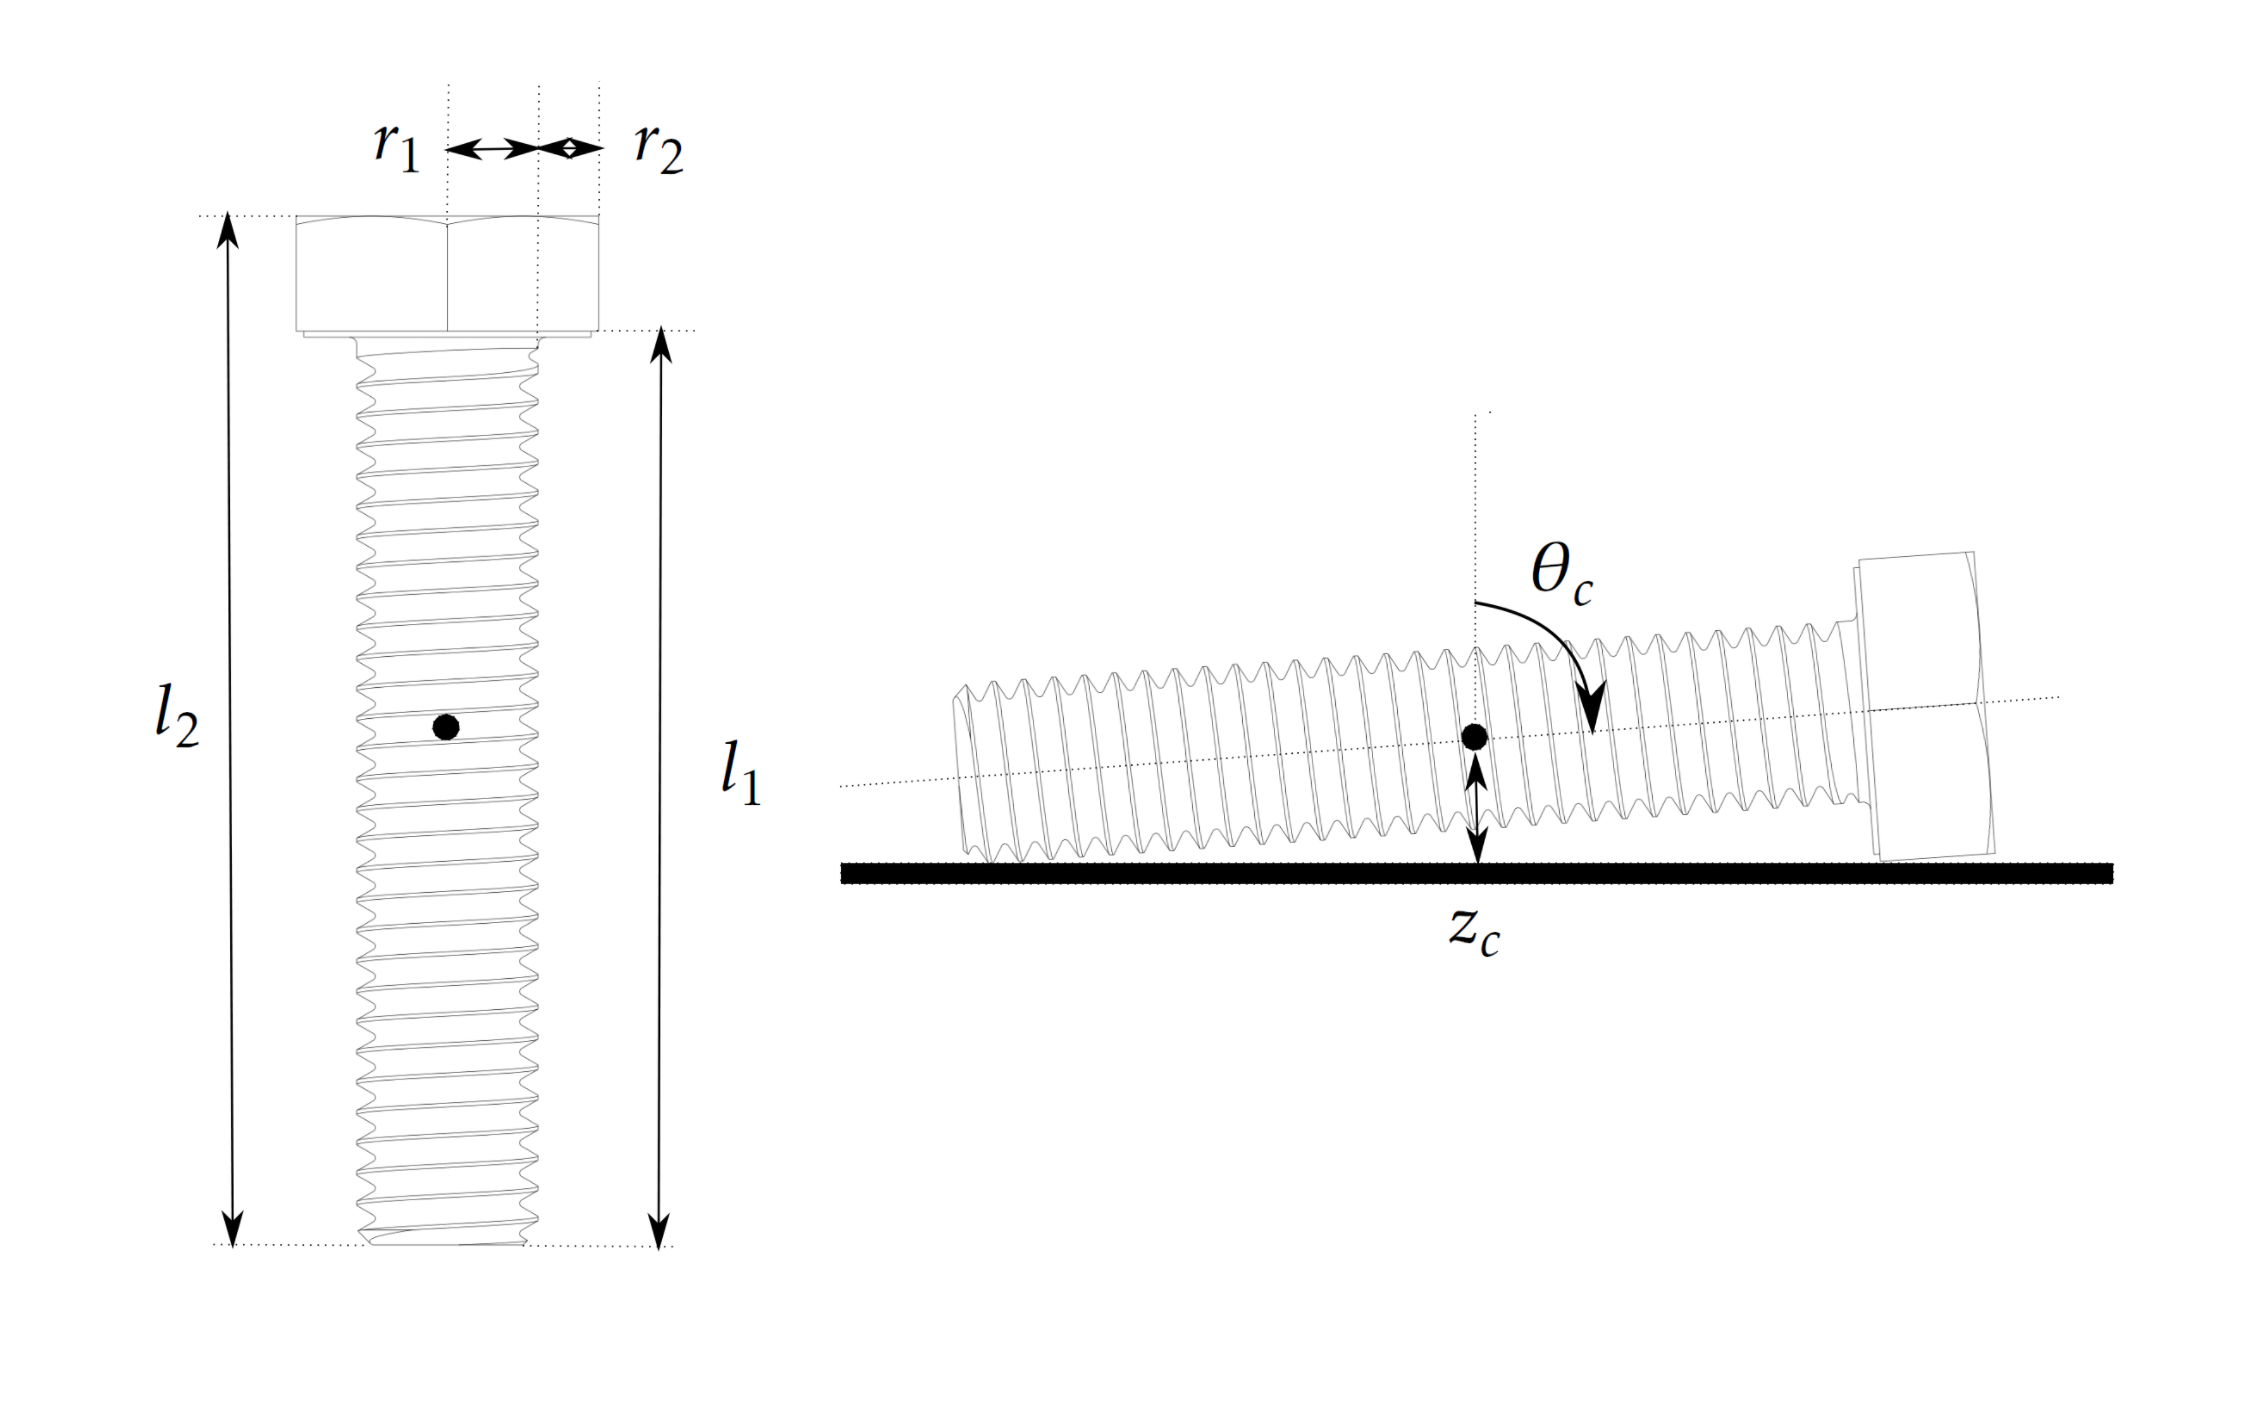
\includegraphics[width=0.8\textwidth]{screwdims.png}
    \caption{Dimensions and pose corrections for the M6x30 hexagonal head screw.}
    \label{fig:screwdim}
\end{figure}

\begin{align*}
    \theta_c &= \frac{\pi}{2} - \arctan \frac{r_2}{l_1}\\
    z_c &= r_1 \sin \theta_c + \frac{1}{2} l_2 \cos \theta_c
\end{align*}

One thing to note is that if an object can have multiple positions on the surface, we consequently have multiple correction transformations to choose from. For example, each screw could be on its side or on its head, which implies a choice between two sets of $t_c$, $R_c$.

Once we have the three transformations $(t_s, \text{R}_s)$, $(t_r, \text{R}_r)$ and $(t_s, \text{R}_s)$, the final pose $(t, \text{R})$ in camera reference is computed as:

\begin{align*}
    t &= t_s + \text{R}_s t_r + \text{R}_s \text{R}_r t_c\\
    \text{R} &= \text{R}_s \text{R}_r \text{R}_c
\end{align*}

With this method, for each background we can quickly generate a series of training images with associated ground truths. While we considered the particular situation of a set of objects placed on a flat surface, the three steps of this approach can be applied to other conditions. In general, these steps are:

\begin{enumerate}
    \item The identification of the area of interest, and primary placement inside that area.
    \item A random transformation within the area of interest, dictated by the degrees of freedom present.
    \item A final transformation dictated by the particulars of the object.
\end{enumerate}

\subsection{Training}

\begin{figure}[ht]
    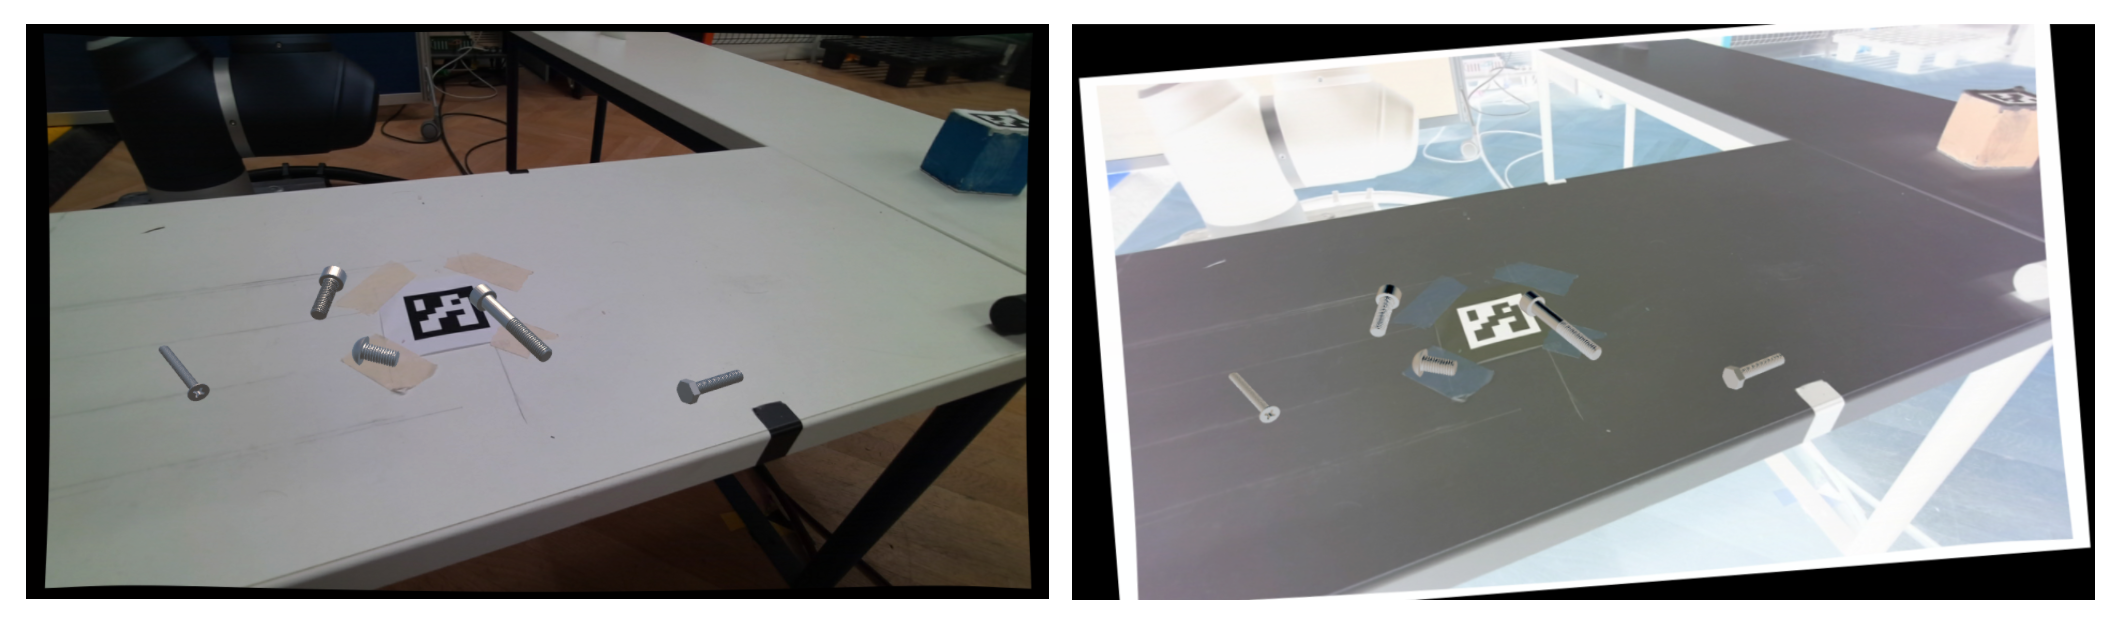
\includegraphics[width=\textwidth]{screwposeaugmented.png}
    \caption{An example of a training image before and after data augmentation.}
    \label{fig:ScrewPoseAugmented}
\end{figure}

The dataset generated with the previous methodology has two major weaknesses. First, there is a limited number of background images, which means that the model has a finite number of camera positions to learn from. This may lead to overfitting and unreliable results for positions that don't have sufficient representation. Second, it is difficult to randomize light intensity and color for the background images inside Unity, as it is decoupled from the same settings for the 3D models.

We can remedy these issues using data augmentation. This is a technique that involves applying random changes to data during training, similarly to how domain randomization would apply them during dataset generation. EfficientPose already provides two data augmentation methods: 6 Degree-of-Freedom augmentation and color augmentation. 6 Degree-of-Freedom augmentation involves randomly rescaling and rotating the input image and consequently adjusting the ground truth, so as to greatly increase the number of possible poses each image can provide. Color augumentation instead implements RandAugment\cite{RandAugment} to change the color and grain for the entire image. Applying both these methods results in images such as the one depicted in figure \ref{fig:ScrewPoseAugmented}, conveniently fixing the issues of our dataset.

Other training parameters are identical to the previous attempt with the fully generated dataset: 100 epochs, with an 80\% learning rate reduction if the model stagnates for 5 epochs.

\subsection{Results}

\begin{table}[ht]
    \begin{center}
        \begin{tabular}{|c||c|c|c|}
            \hline
            Object & AP & AD-S [mm] & ADD-S \\
            \hline \hline
            M6x30 & 0.9399 & 2.1434 & 82.30\% \\
            M8x16 & 0.9538 & 1.9988 & 67.54\% \\
            M8x25 & 0.9645 & 2.1179 & 85.07\% \\
            M8x50 & 0.9880 & 3.4482 & 93.30\% \\
            \hline \hline
            Average & 0.9615 & 2.4271 & 82.05\% \\
            \hline    
        \end{tabular}
        \caption{Evaluation of the Average Precision, Average Symmetric Distance, and ADD-S metrics on the augmented reality dataset after training.}
        \label{tab:screwpose}
    \end{center}
\end{table}

After training, the progress of which can be seen in figure \ref{fig:screwpose_training}, the model achieves the results shown in table \ref{tab:screwpose}.

Overall, the performance of this model is much better than the previous one, obtaining an average ADD-S of 82.05\%, which is better than EfficientPose's reported 79.04\% on Occlusion-LINEMOD with $\phi=0$, and comparable to its 83.98\% with $\phi = 3$. This is a good result, considering that the objects for our dataset are smaller, symmetric and all visually similar.

Furthermore, the model is capable of generalising to real life situations without noticeable decreases in performance, as can be seen in figure \ref{fig:screwpose_inferencing}.

\begin{figure}[ht]
    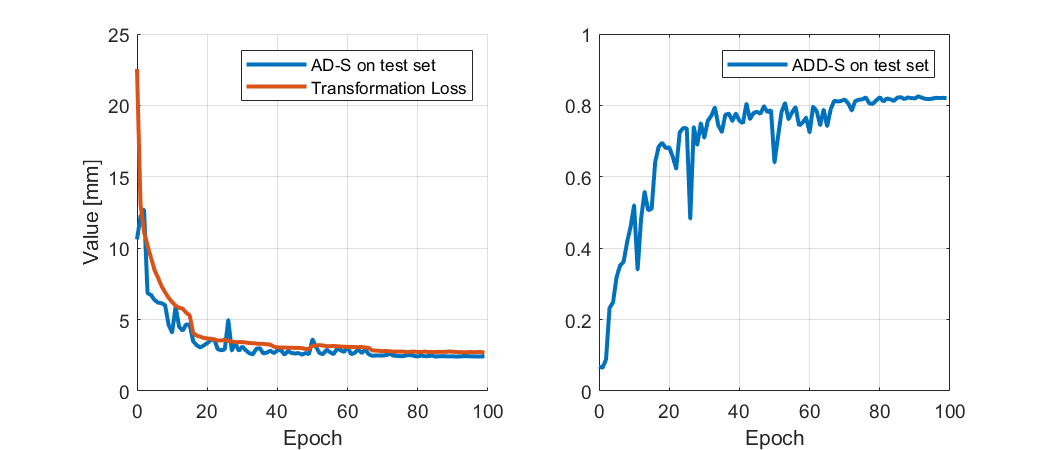
\includegraphics[width=\textwidth]{screwpose_training.png}
    \caption{Evolution of the loss, AD-S and ADD-S metrics during training for the partially rendered dataset. The loss is computed as the AD-S metric on the training dataset.}
    \label{fig:screwpose_training}
\end{figure}

\begin{figure}[ht]
    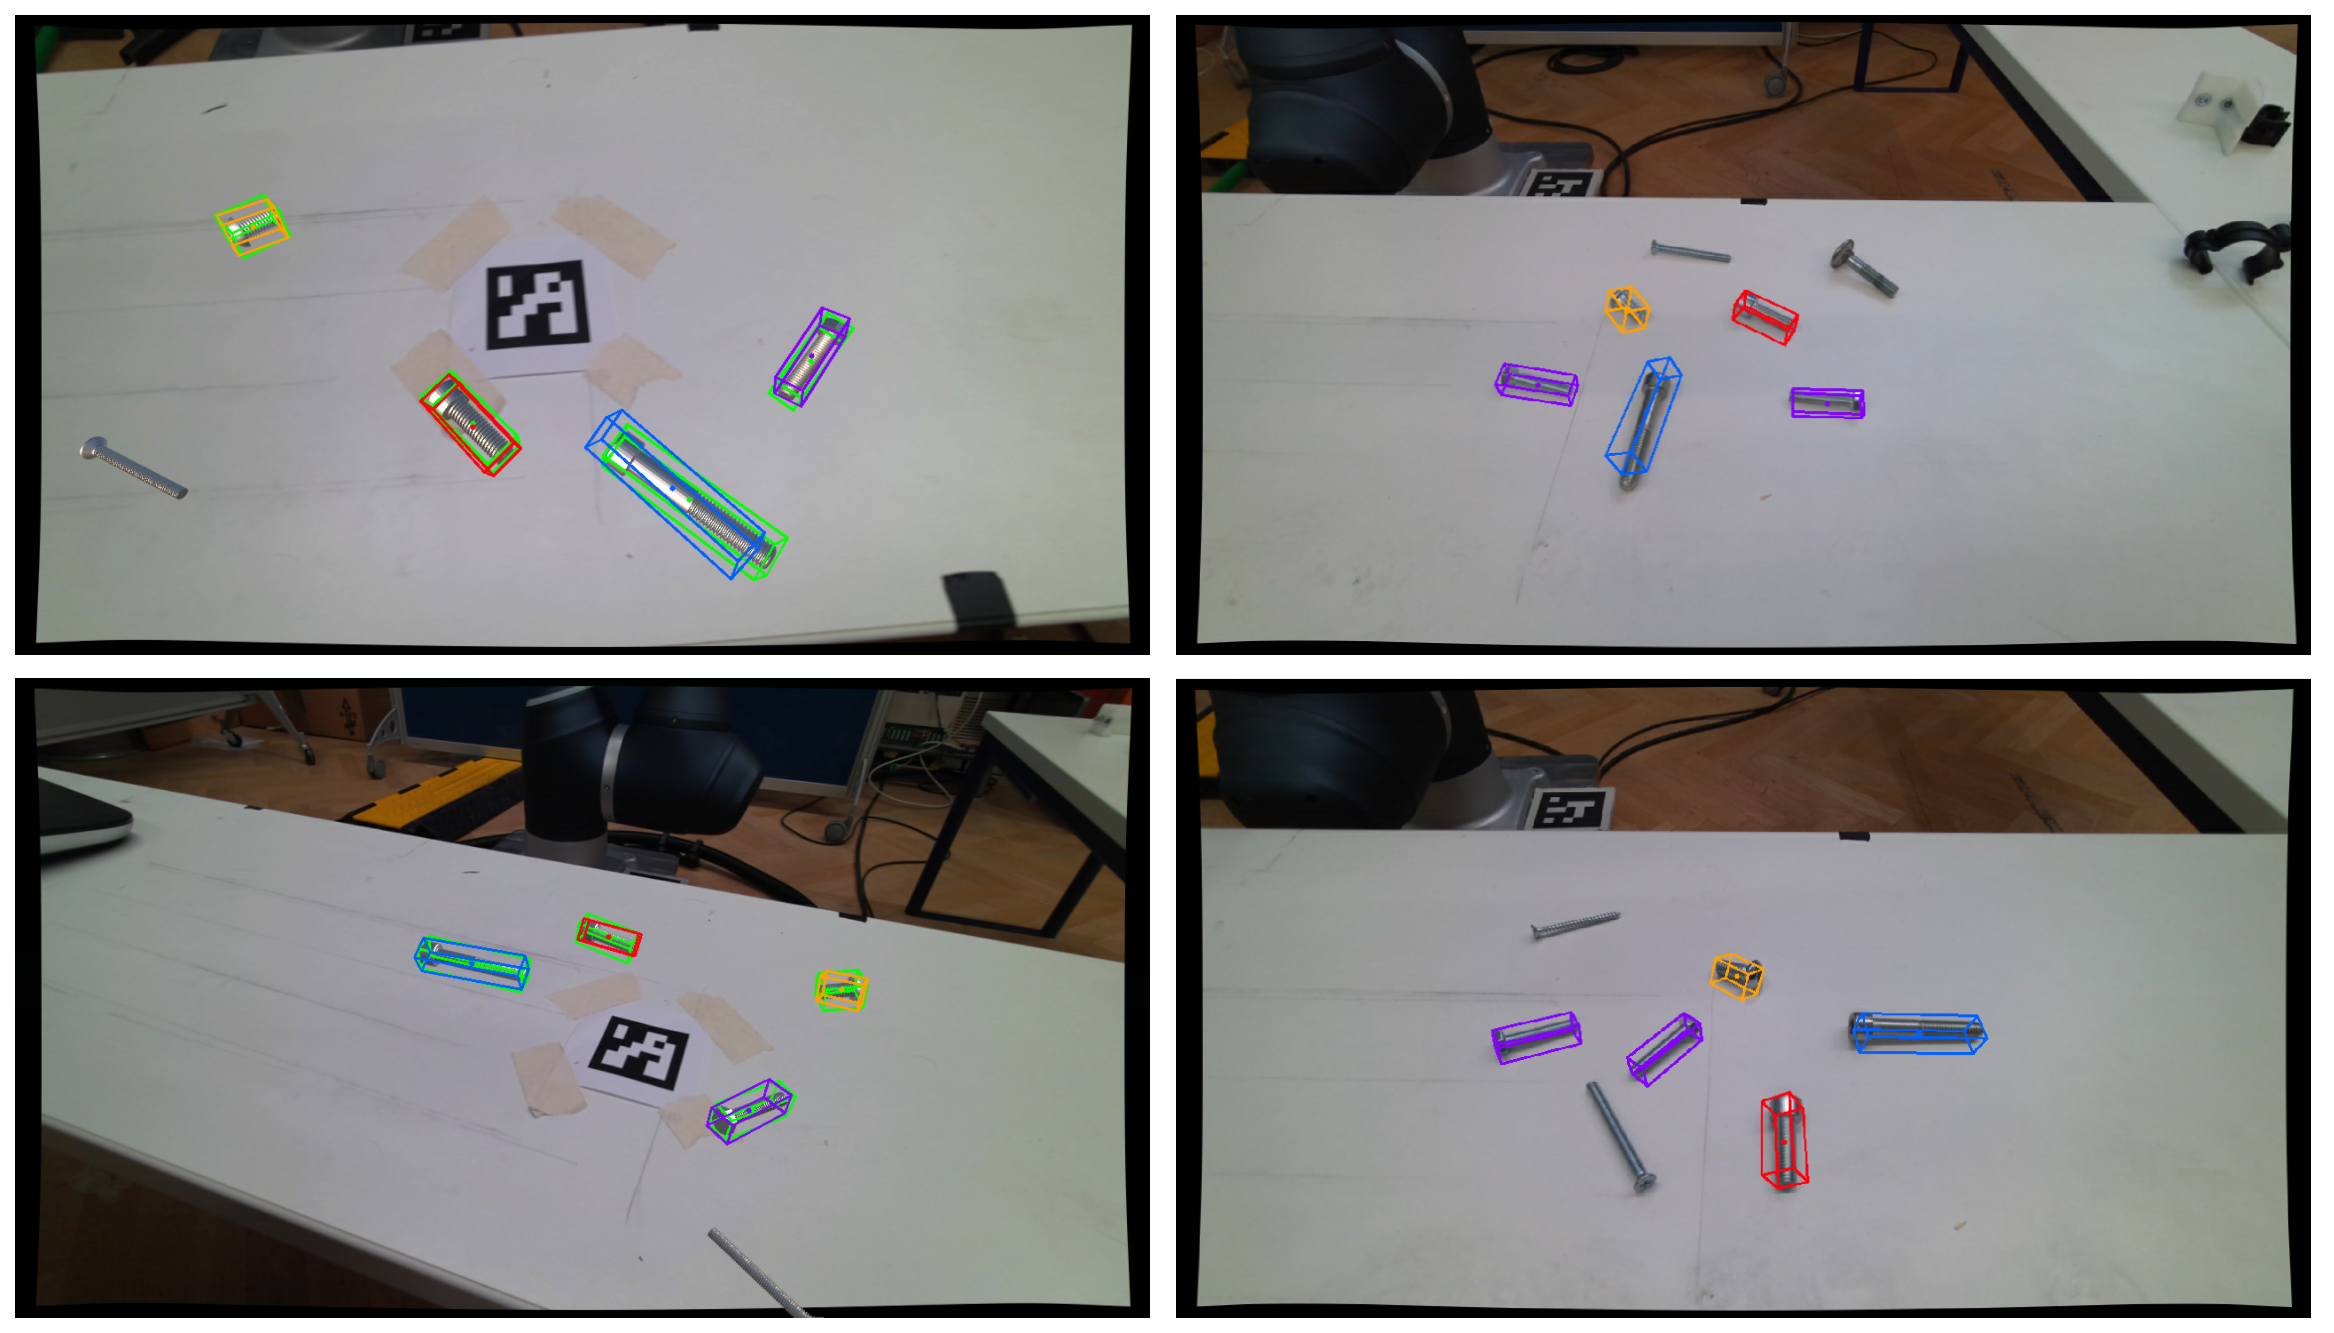
\includegraphics[width=\textwidth]{screwpose_inferencing.png}
    \caption{Four images displaying pose estimations from the network for the augmented reality dataset. The left two are part of evaluation and display ground truths with green bounding boxes, the right two are captures from a real camera in the testing environment.}
    \label{fig:screwpose_inferencing}
\end{figure}

\section{Semantics Applications}

\subsection{Motivations and Objective}

In many applications, it may be that estimating the pose of an object is sufficient to perform the task. However, it it often necessary to infer additional information from this data. A typical situation is the assembly of a workpiece from its components, where while tracking the pose of each individual component we may also have to track the state of the assembly itself.

Thus we want to ascertain if it is viable to use pose estimation techniques to track the position of the components for an assembly task, and simultaneously obtain information of its overall state.

\subsection{Dataset Generation and Training}

The first step to working with neural networks is again the generation of the datasets required for training and evaluation. For our task, we are considering the assembly of a set of modular button boards. We have two boards, one with two slots, and one with three slots. These slots can be filled in any order with one of three buttons: a larger safety button, and two smaller buttons with different designs on their faces, but identical shape. The CAD models for these objects were available online from the supplier's website, and we used Blender to color them appropriately. Renders for these objects are depicted in figure \ref{fig:buttonpose_objects}.

\begin{figure}[ht]
    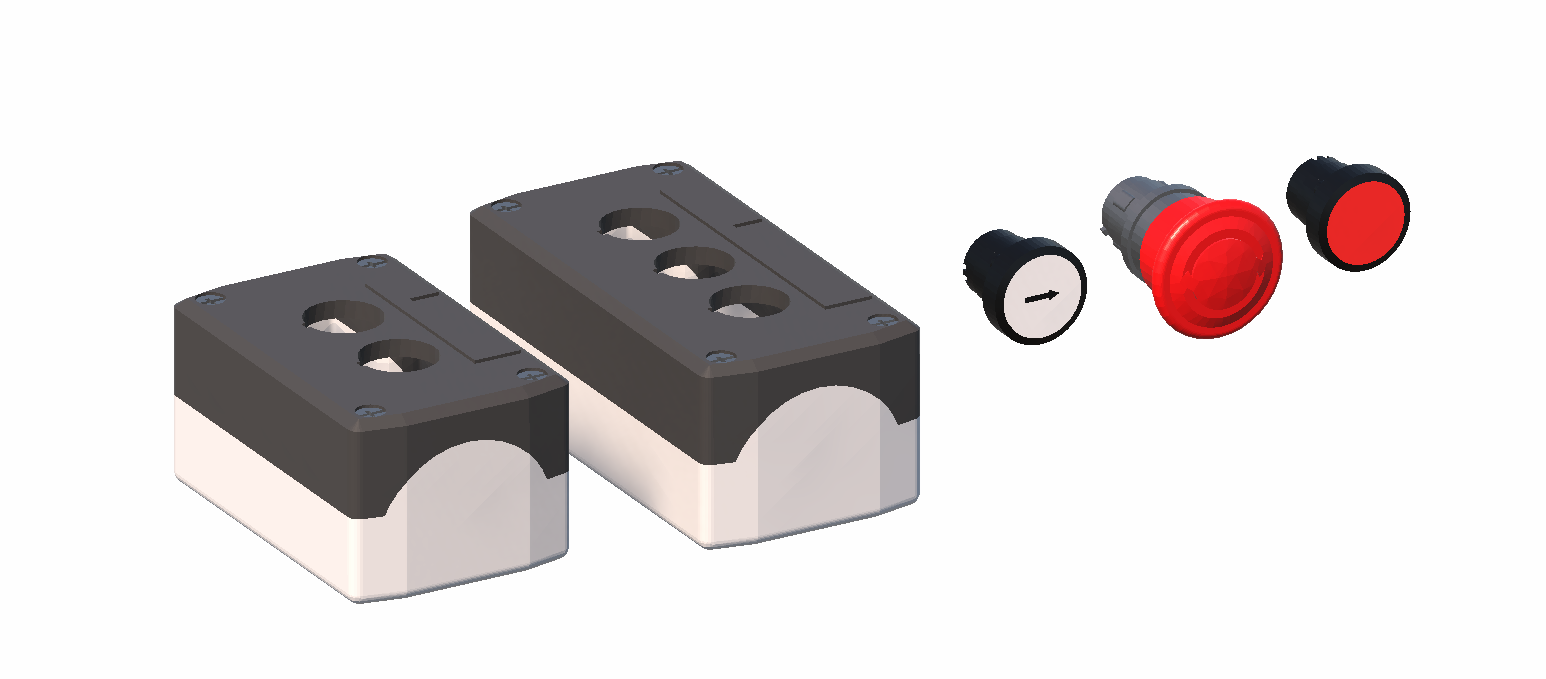
\includegraphics[width=0.6\textwidth]{buttonpose_objects.png}
    \caption{Orthographic rendering of dataset objects: two modular button boards and three buttons.}
    \label{fig:buttonpose_objects}
\end{figure}

To generate the dataset images we can use the same method used for the Augmented Reality dataset, however we have a few noticeable differences that require consideration. The first obvious one is that we would like to represent the buttons not only while they are freely placed on the table surface, but also when they are slotted into a board. This is achievable by positioning the button with the same pose as the board, and then applying a final roto-translation that shifts the button into a slot. We can compute these transformations in advance and simply apply them when necessary.

One important thing to note is that these roto-translations depend on the shape of the button: thus the safety button will require different values compared to the other two.

The second, more insidious issue has to do with the two smalle buttons with identical shape. These buttons are distinguishable only by the different designs on their faces, but when placing them randomly, there is a good chance that these faces are not visible. This leads to a situations where it is impossible to differentiate between the two, causing a drastic drop in performance, as during training the network will percieve a large number of false positives.

To solve this issue, we can add a fictional object to the dataset, the "unidentified button". Simply put, we categorize buttons without their unique face visible as a new object class, since it is impossible for the network to directly identify them as one type or the other.

\begin{figure}[ht]
    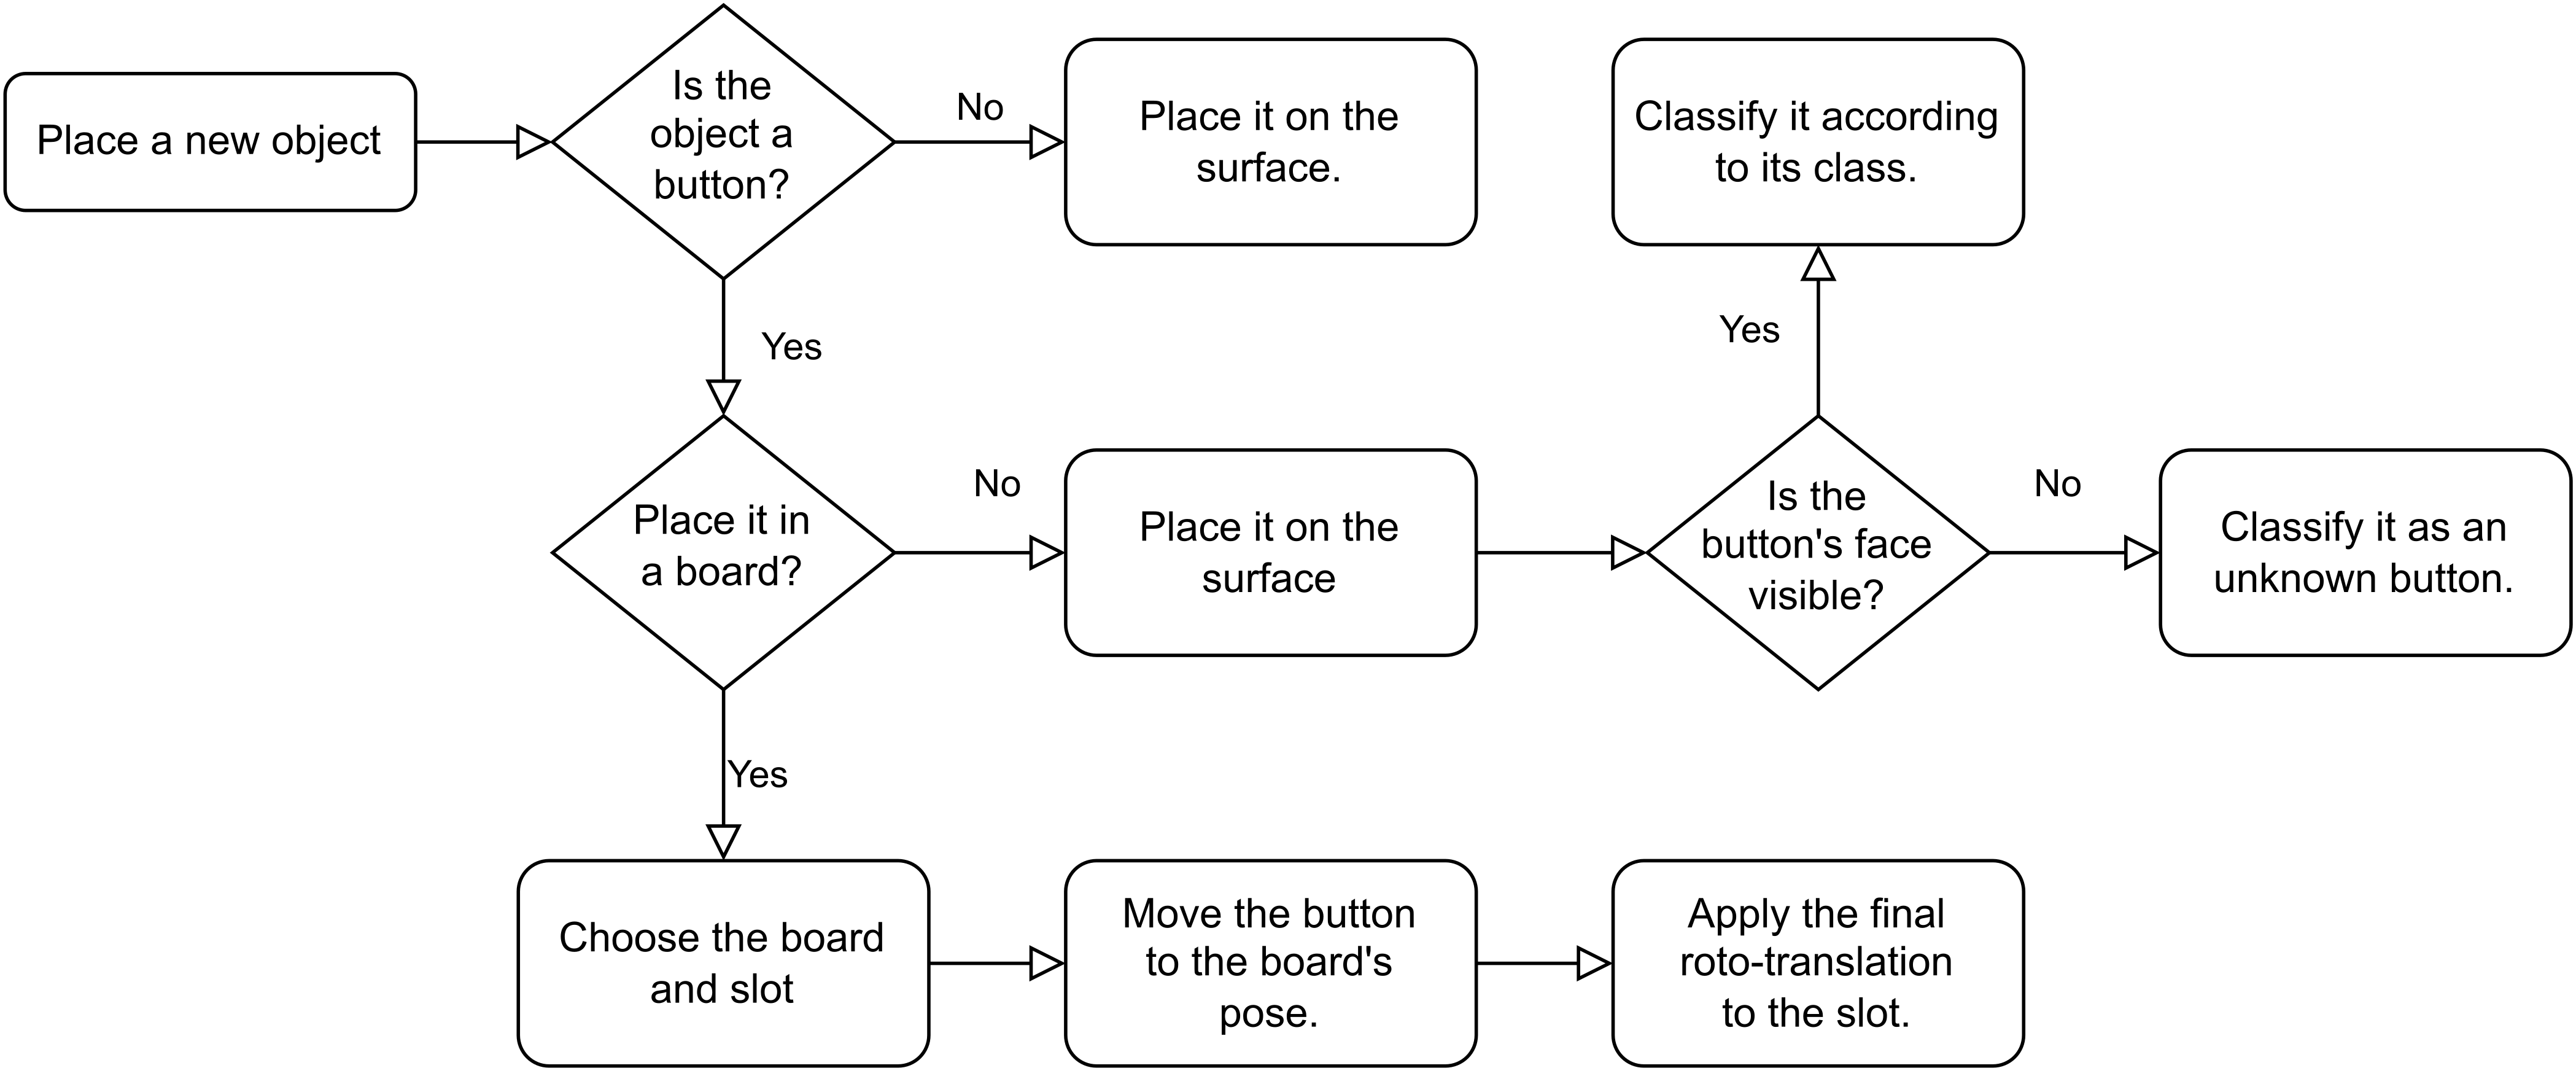
\includegraphics[width=\textwidth]{buttonpose_placement.png}
    \caption{Flowchart representing the algorithm for placement of dataset objects, when placing buttons inside of slots and checking for face occlusion.}
    \label{fig:buttonpose_placement}
\end{figure}

We can use a simple geometric method to determine if a button's face is visible during generation, explicated in figure \ref{fig:button_occlusion}. Considering the origin of the camera reference frame $O = [0, 0, 0]^T$, the button's pose is given by the translation vector $t$ and the rotation matrix R. $t$ also indicates the position of the center of the button $C$, due to it being the origin of the button's 3D model. If we then consider the vector $f = [f_x, f_y, f_z]^T$ indicating the position of the center of the button's face $F$ in the button's frame of reference, the position of this point in the camera frame is given by:

\begin{figure}
    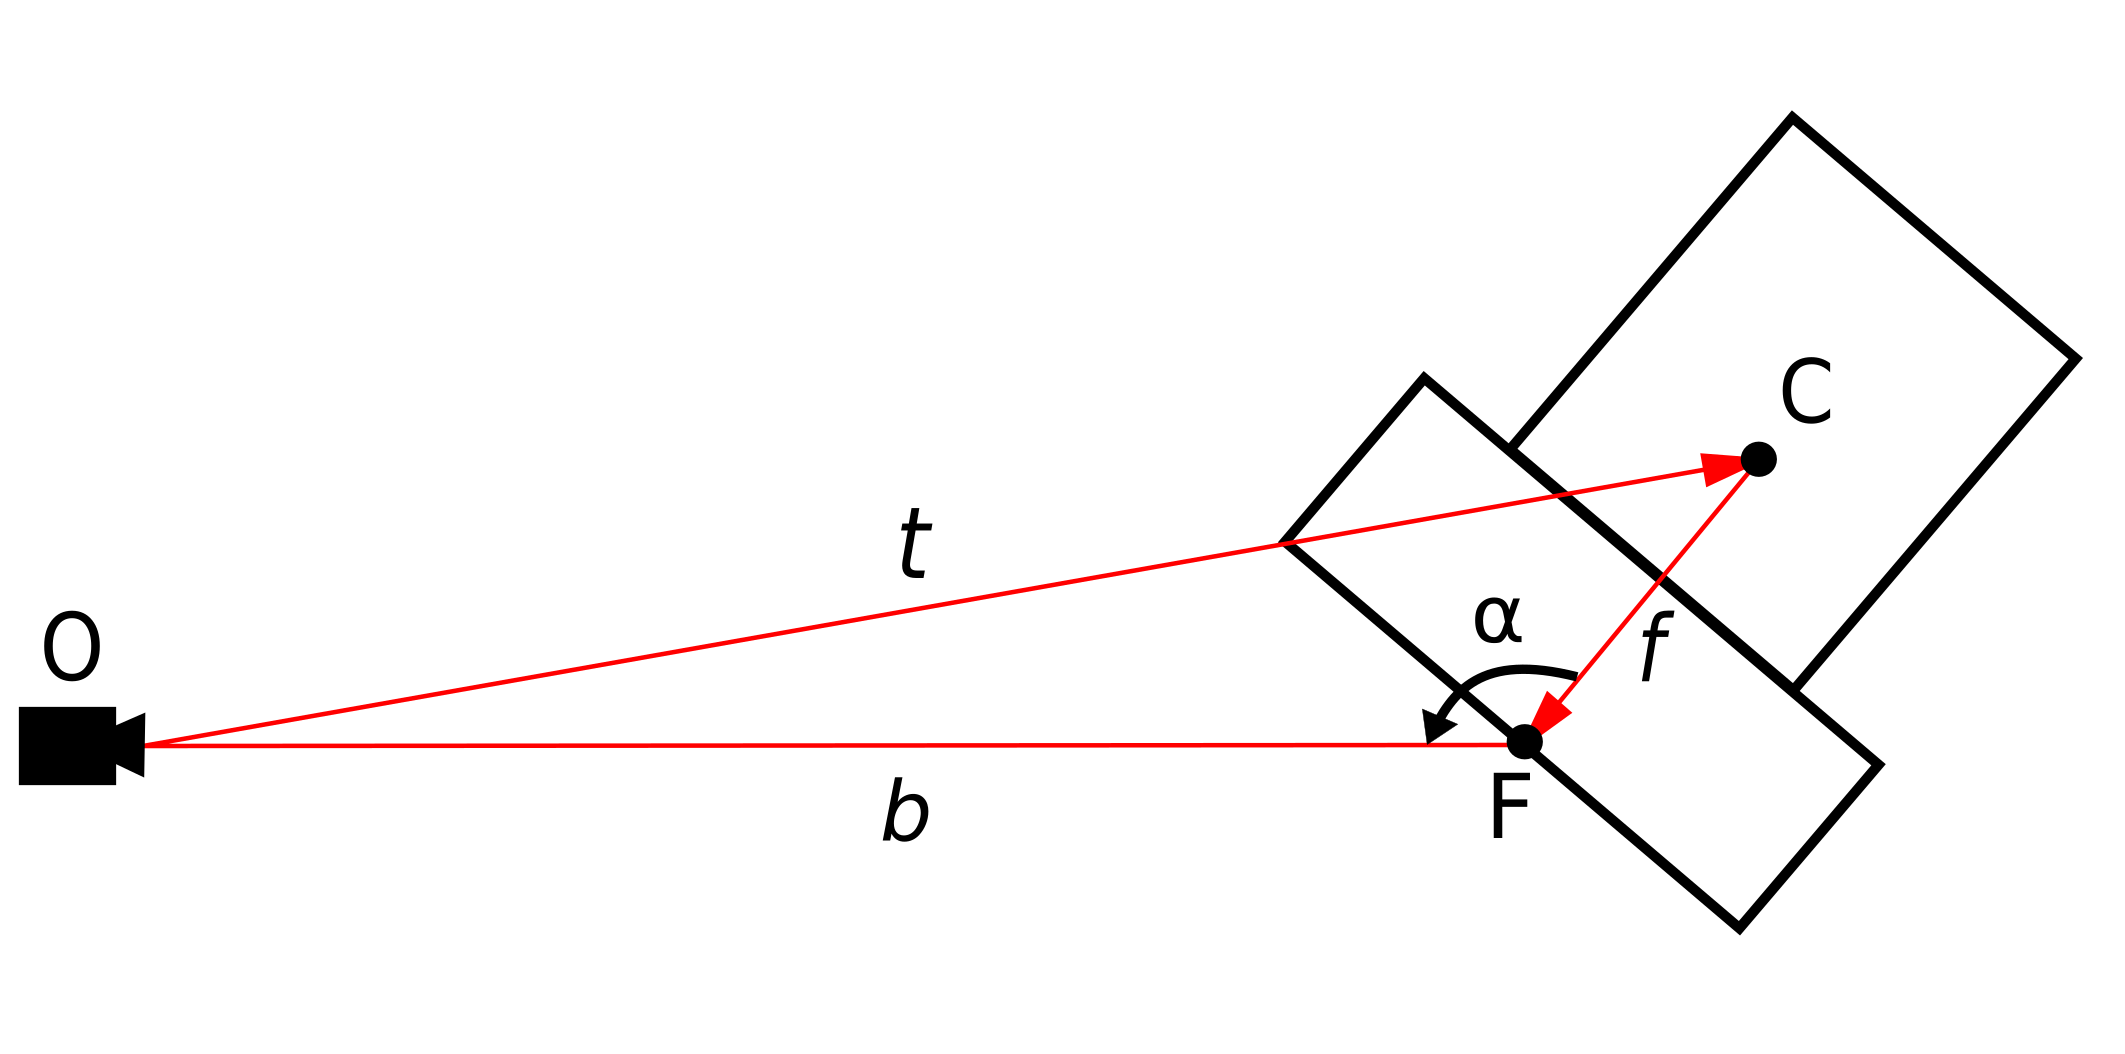
\includegraphics[width=0.7\textwidth]{button_occlusion.png}
    \caption{Schematic representation of the button relative to the camera, and of the variables used when evaluating occlusion of the button face.}
    \label{fig:button_occlusion}
\end{figure}

\begin{equation*}
    F = t + \text{R}f
\end{equation*}

We can then compute the amplitude of the angle $\alpha = C\hat{F}O$. Denoting $OF=b$, we apply the law of cosines:

\begin{equation*}
    t^Tt = b^Tb + f^Tf -  2||b||\cdot ||f|| \cdot \cos \alpha
\end{equation*}

By making $\alpha$ explicit in this equation we obtain:

\begin{equation*}
    \alpha = \cos^{-1}\left(\frac{t^Tt- b^Tb-f^Tf}{2||b||\cdot||f||}\right)
\end{equation*}

It is simple to verify geometrically that the button's face is occluded whenever $\alpha < 90\degree$, and viceversa. To avoid strange edge cases where the button's face is barely visible in the proximity of $\alpha = 90\degree$, we introduce a small buffer angle $\beta$, usually around 5\degree. Thus we categorize a button as unrecognizeable whenever $\alpha < 90\degree + \beta$, overwriting its class in the ground truths with the "unknown button" class.

Thus we have a method for creating arbitrarily large datasets for our application. We decided to generate 20'000 images, where 18'000 are used for training and 2'000 for verification. Therefore we reduced the number of epochs to 40, and the patience for learning rate reduction to 3 epochs. All other parameters are identical to our previous attempts.

\begin{figure}
    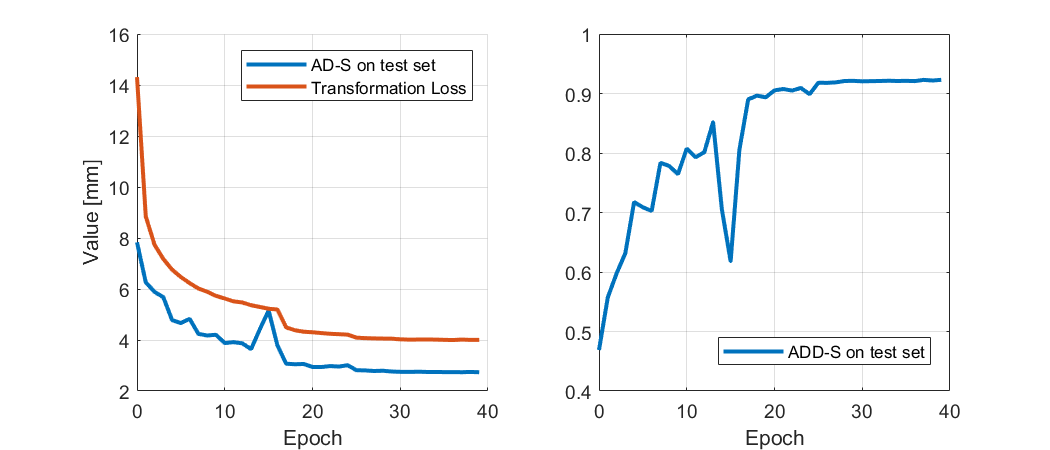
\includegraphics[width=\textwidth]{buttonpose_training.png}
    \caption{Evolution of the loss, AD-S and ADD-S metrics during training for the partially rendered dataset. The loss is computed as the AD-S metric on the training dataset.}
    \label{fig:buttonpose_training}
\end{figure}

\begin{table}[ht]
    \begin{center}
        \begin{tabular}{|c||c|c|c|}
            \hline
            Object & AP & AD-S [mm] & ADD-S \\
            \hline \hline
            2-slot & 0.9990 & 3.5420 & 99.90\% \\
            3-slot & 0.9985 & 3.9304 & 99.85\% \\
            red button & 0.9260 & 1.9825 & 86.01\% \\
            arrow button & 0.9349 & 2.0497 & 86.05\% \\
            safety button & 0.9962 & 2.6053 & 98.01\% \\
            unknown button & 0.9561 & 2.4757 & 82.95\% \\
            \hline \hline
            Average & 0.9685 & 2.76 & 92.13\% \\
            \hline    
        \end{tabular}
        \caption{Evaluation of the Average Precision, Average Symmetric Distance, and ADD-S metrics on the buttons dataset after training.}
        \label{tab:buttonpose}
    \end{center}
\end{table}

Training resulted in abnormally good performance for the boards, reaching over 99\% ADD-S and AP for both. The larger safety button also obtained great results, with a 98\% ADD-S, while the other buttons achieved more middling performances, but still better than the 79.04\% ADD benchmark repored on Occlusion-LINEMOD.

\begin{figure}[ht]
    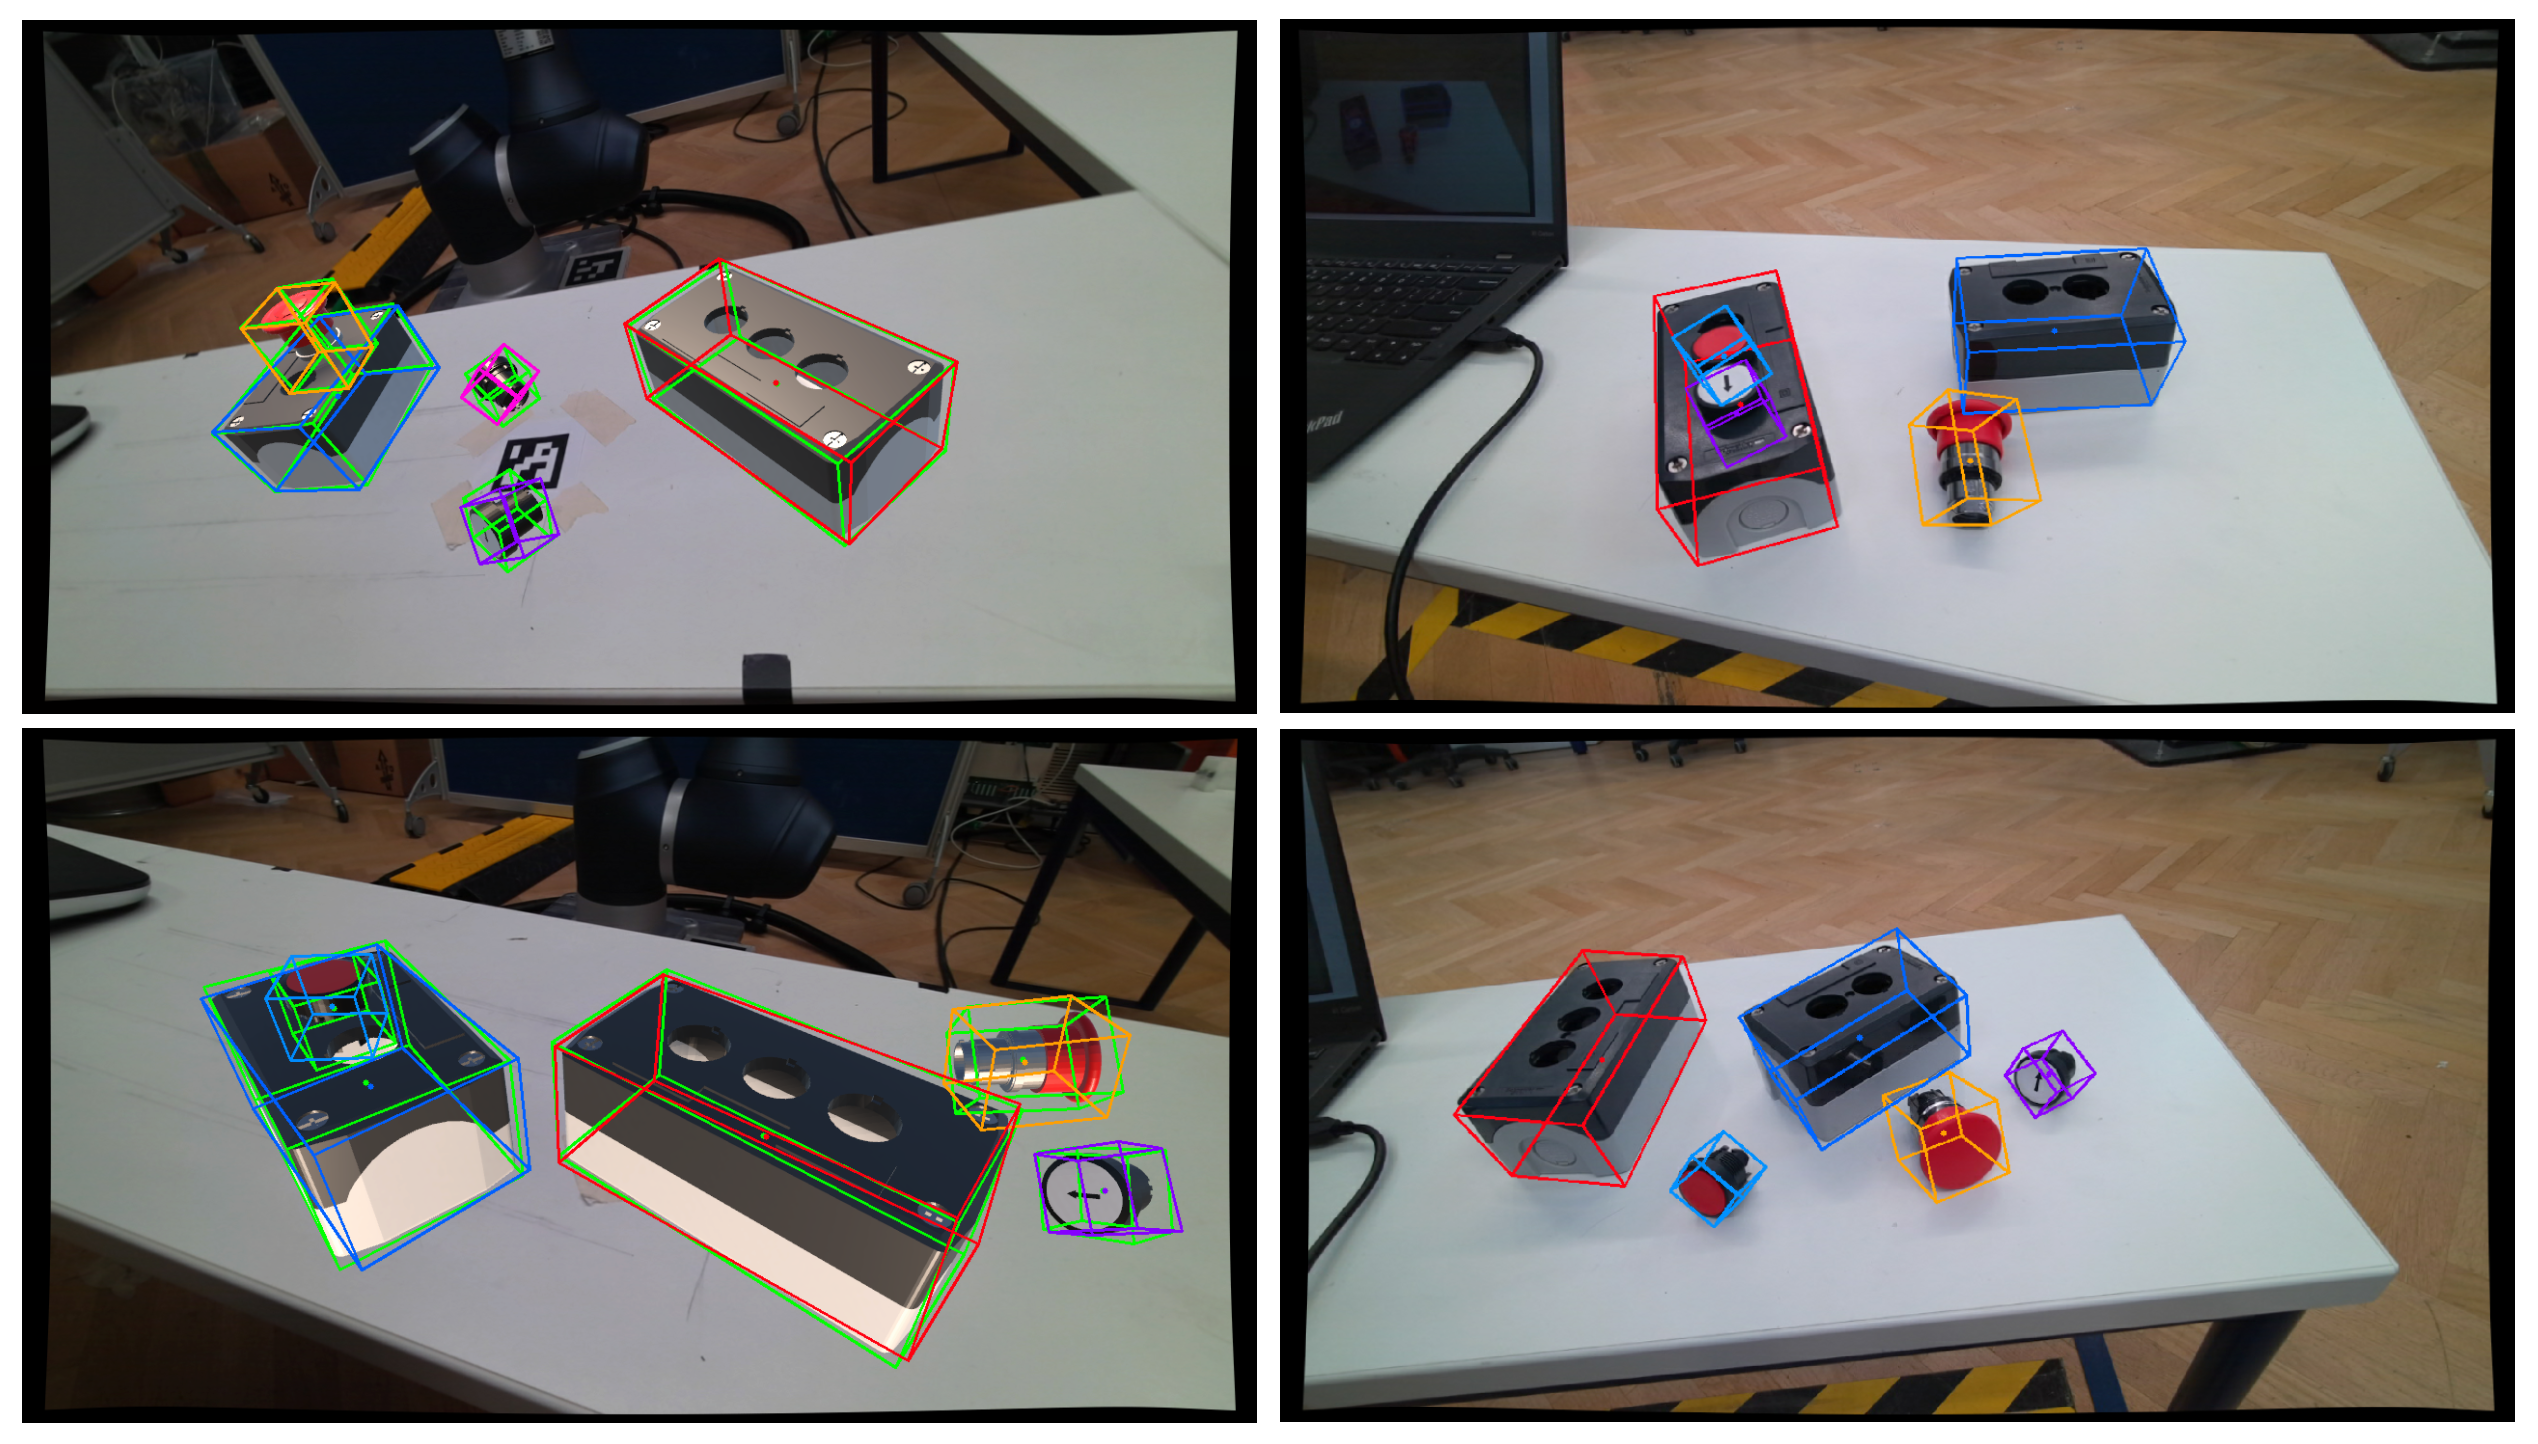
\includegraphics[width=\textwidth]{buttonpose_inferencing.png}
    \caption{Four images displaying pose estimations from the network for the button dataset. The left two are part of evaluation and display ground truths with green bounding boxes, the right two are captures from a real camera in the testing environment.}
    \label{fig:buttonpose_inferencing}
\end{figure}

\subsection{Thresholding}

Now that we have a dataset and a model trained on it, we can begin the task of creating a method to identify the state of the overall assembly. There are two pieces to this assembly: buttons and the boards they're to be slotted in. The problem now becomes: given the position of a button and the position of a board, how does one determine whether the button is slotted into the board, and in which slot?

A simple and intuitive way to handle this problem is through the computation of a distance metric: given a slot and a button, if the "distance" between the two is less than a threshold, we can reasonably affirm that the button is in the slot. We considered two different distance metrics for this task: center-to-center distance and average symmetric distance.

Center-to-center distance is the distance between the estimated position of the center of the button $C$, and the position this center would have if the button was already in the slot, $C'$, as depicted in figure \ref{fig:center2center}. While the first position is a direct output of our network, the second one must be obtained from the succession of three roto-translations: one from the camera reference to the position of the board, which is a direct output of the network; a second to the position of the slot relative to the board, which is known for each slot; and the last one from the position of the slot to the position of the hypothetical button center, which varies based on the geometry of the button.

\begin{figure}[ht]
    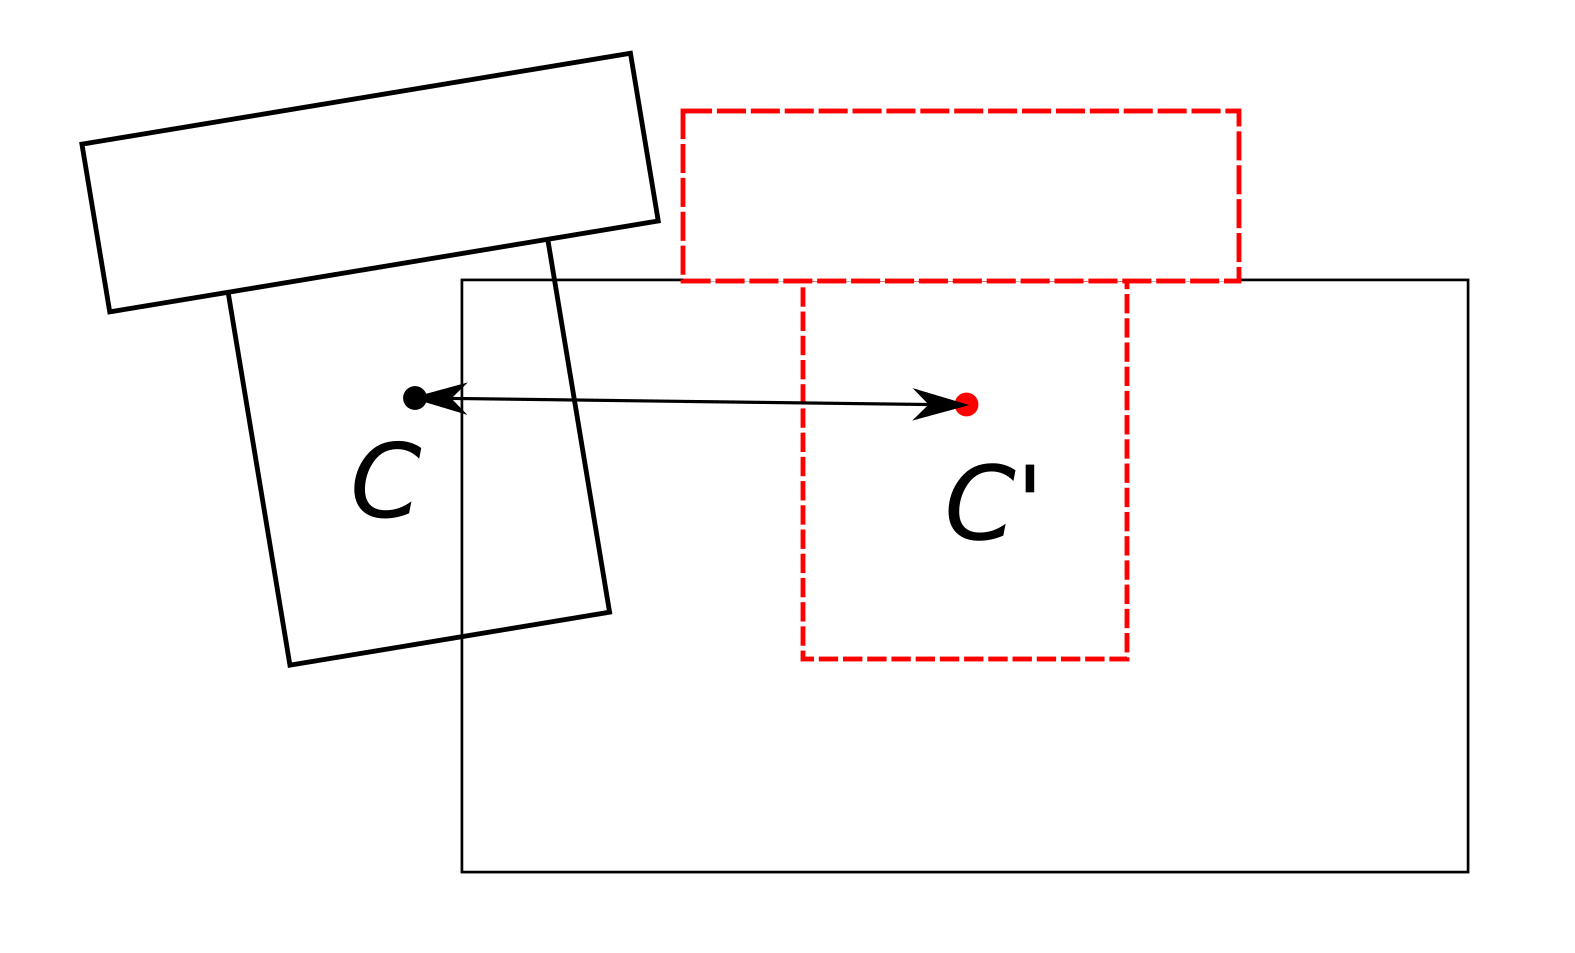
\includegraphics[width=0.6\textwidth]{Center-to-center.png}
    \caption{Depiction of the center-to-center distance from a button to a slot. In black is the estimated pose of the button, while in red is the estimated position of a button if it was hypothetically already in the slot.}
    \label{fig:center2center}
\end{figure}

The average symmetric distance is instead identical to the AD-S computed as a metric during training and evaluation. Considering again the estimated pose of the button $(\text{R}, t)$ and the pose the button would have if it was considered in the slot $(\text{R}', t')$, the average distance is computed as:

\begin{equation*}
    \text{AD-S} = \frac{1}{n} \sum_{x_1 \in M} \min_{x_2 \in M} ||(\text{R}x_2 + \text{t}) - 
    (\text{R}'x_1 + \text{t}')||_2
\end{equation*}

... where M is the set of the points composing the button's 3D model, and n is the number of points considered. While this metric has the advantage of considering differences in rotation, which center-to-center is unable to do, it is also much more demanding computationally, depending on the number of points considered.

However, these metrics alone are insufficient to solve our problem. This is because, since each slot is in close proximity with others, for higher thresholds there will be conflicts where multiple slots are within range of the same button or multiple buttons are in range of the same slot, as depicted in figure \ref{fig:conflicts}.

\begin{figure}[ht]
    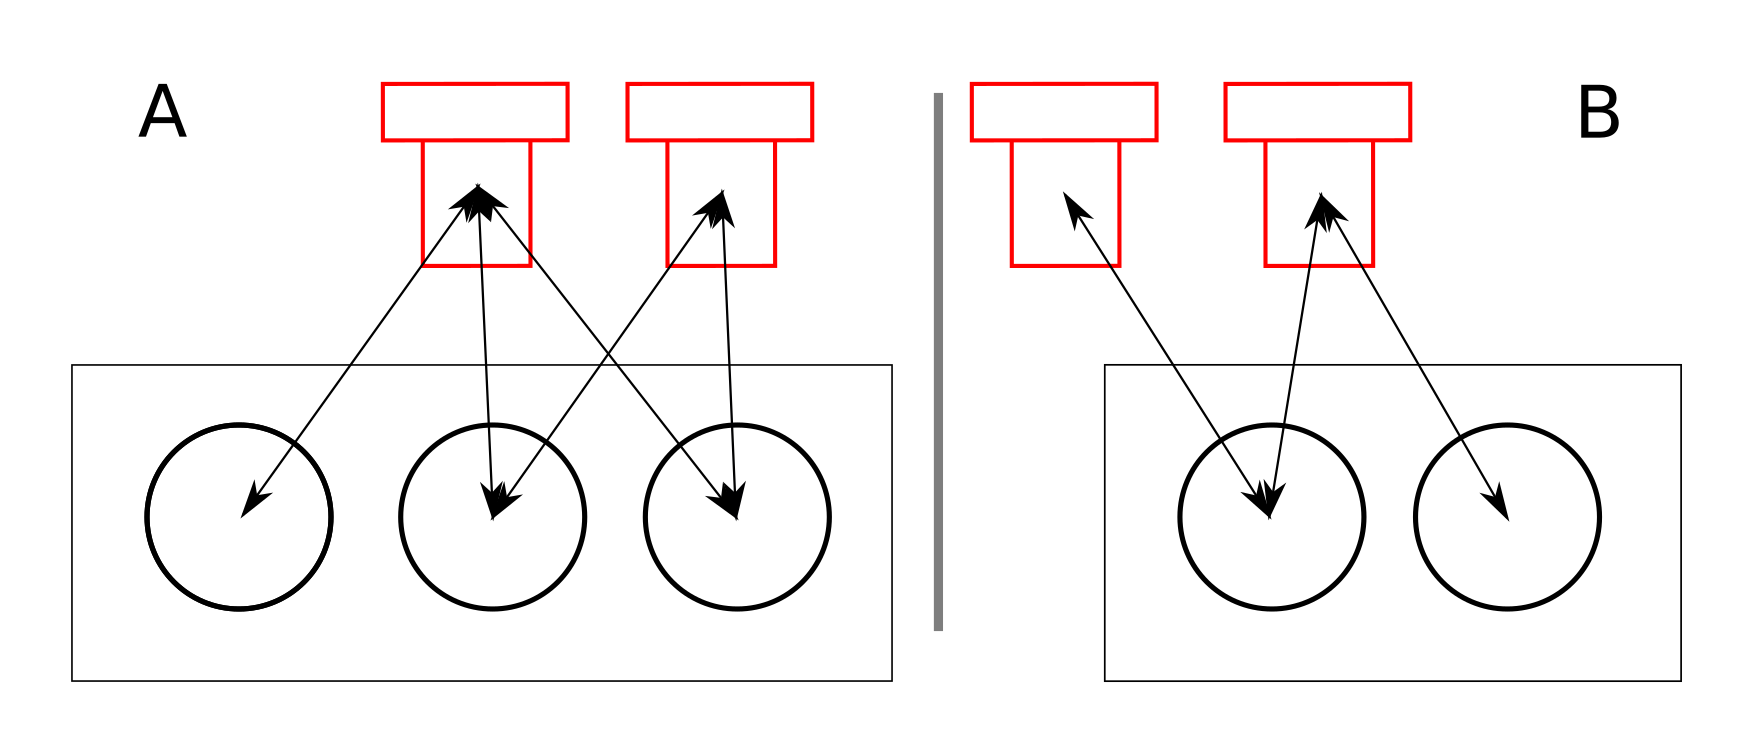
\includegraphics[width=0.8\textwidth]{buttons_conflict.png}
    \caption{Schematic depiction of two hypothetical situations that would generate conflicts by placing multiple buttons within the threshold of a single slot or vice-versa.}
    \label{fig:conflicts}
\end{figure}

To resolve these conflicts, we introduce an intuitive "double check" method that provides excellent results with minimal complexity. This method requires three steps:

\begin{enumerate}
    \item For each button, we assign it to the closest slot within the threshold, if there is one.
    \item For each slot, we assign it to the closest button within the threshold, if there is one.
    \item For each assignment, it is confirmed only if it is reciprocated, and otherwise it is ignored.
\end{enumerate}

An assignment from a slot to a button is considrered reciprocated only if the button is also assigned to the slot, and vice-versa

\begin{figure}[ht]
    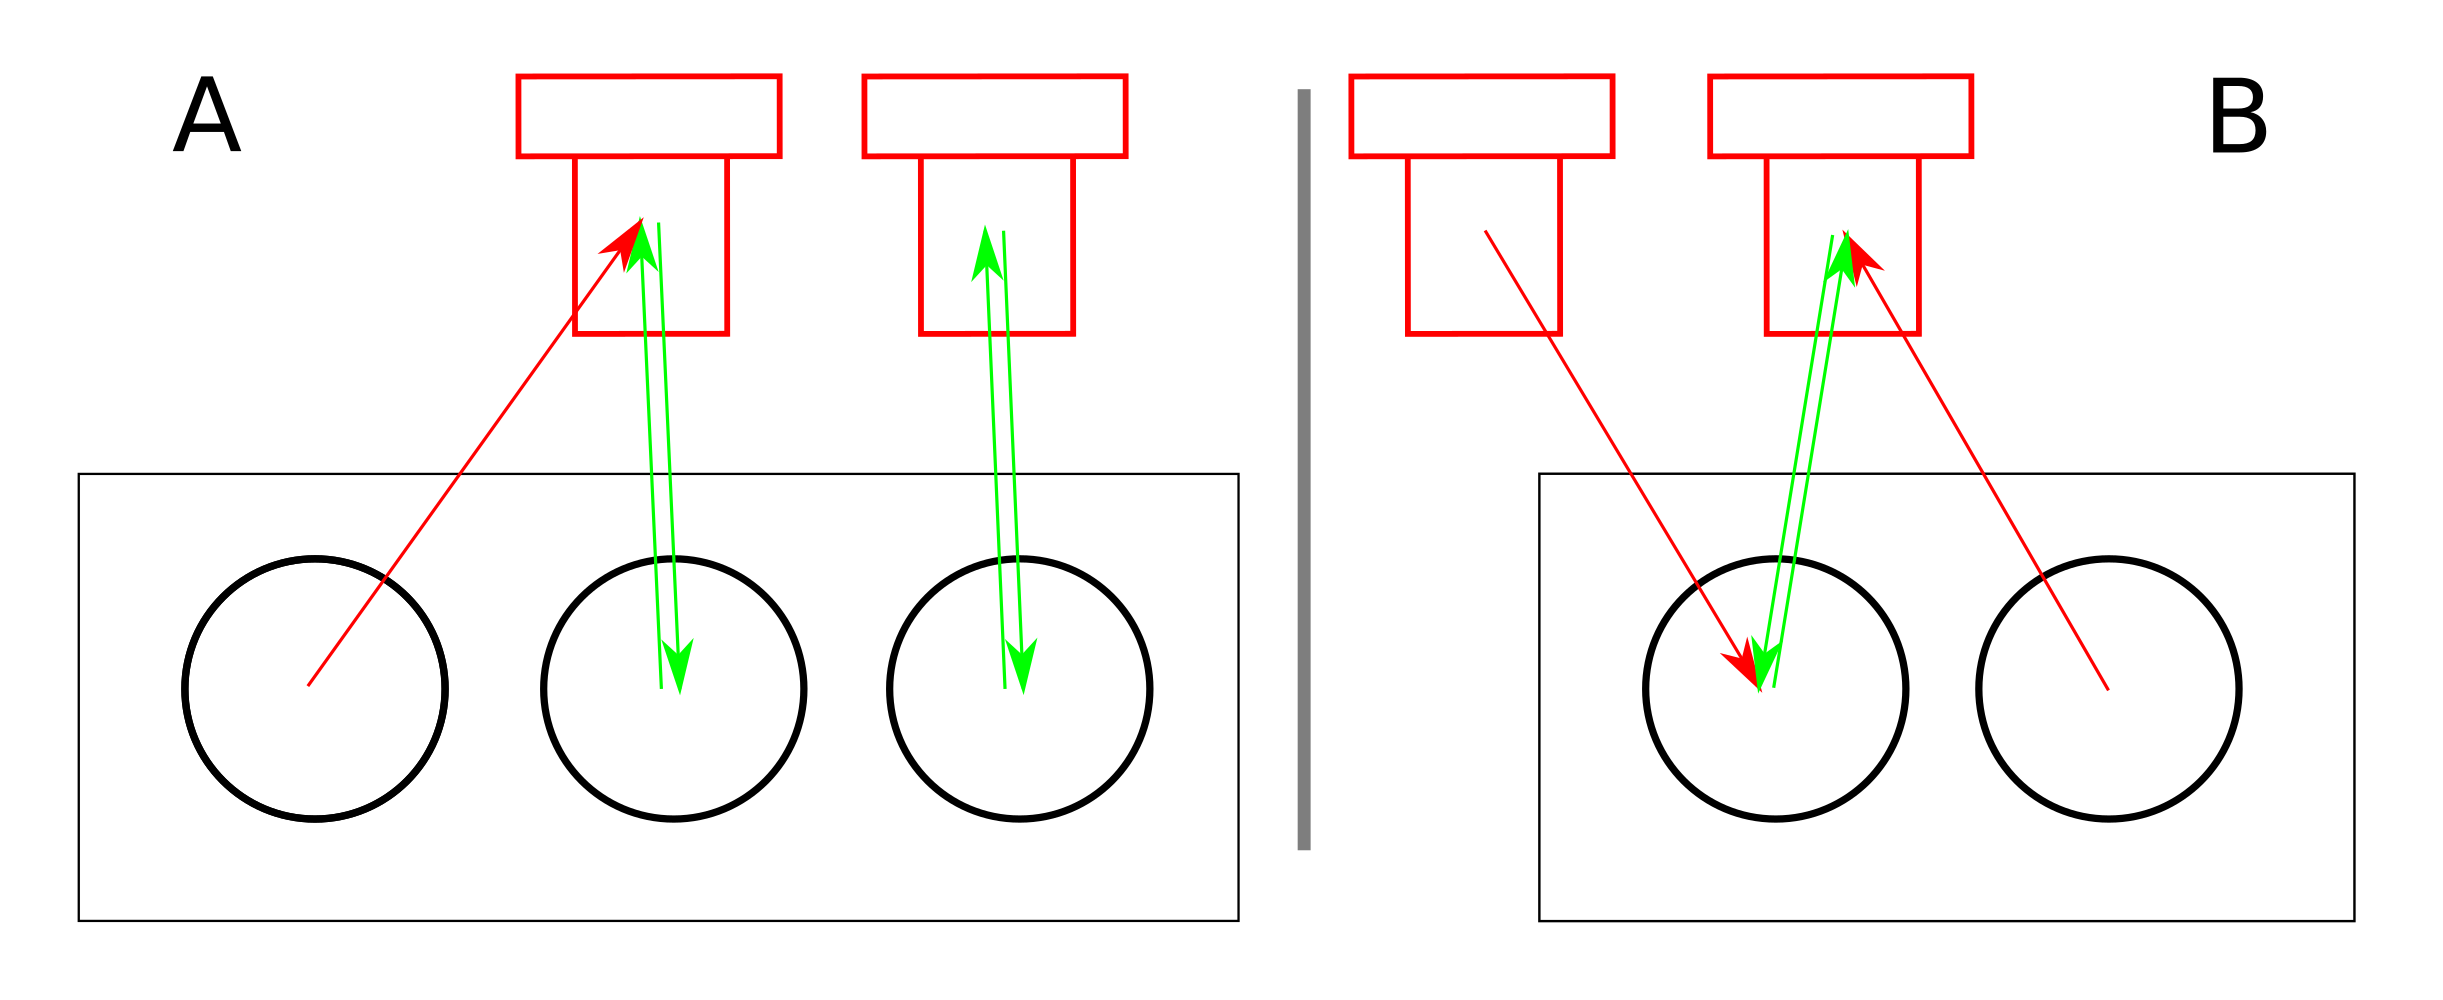
\includegraphics[width=0.8\textwidth]{buttons_resolution.png}
    \caption{Schematic depiction of the resolution of the conflicts previously depicted in figure \ref{fig:conflicts}. Green arrows represent reciprocating assignments, which are confirmed, while red arrows represent non-reciprocating assignments, which are ignored.}
    \label{fig:resolution}
\end{figure}

Now that we have a way to resolve conflicts, we must select the optimal threshold that maximises the performance of our method. To do this we will use the concepts of precision and recall applied to our generated dataset. Given a binary classification problem such as ours (a button can either be in a slot or not), based on the output of our method we can build a confusion matrix as shown in table \ref{tab:cmatrix}.

\begin{table}[ht]
    \begin{center}
        \begin{tabular}{c||c|c}
            \space & Actual Positives & Actual Negatives\\
            \hline\hline
            Predicted Positives & True Positives (TP)& False Positives (FP)\\
            \hline
            Predicted Negatives & False Negatives (FN)& True Negatives (TN)\\
        \end{tabular}
        \caption{Generation of the confusion matrix.}
        \label{tab:cmatrix}
    \end{center}
\end{table}

From these values, precision and recall are defined as:

\begin{align*}
    \text{Precision} =& \frac{\text{TP}}{\text{TP}+\text{TN}} \\
    & \\
    \text{Recall} =& \frac{\text{TP}}{\text{TP}+\text{FN}}
\end{align*}

We want to maximise both of these metrics. To do this, we can plot them as a function of the threshold, and as a function of each other in a precision-recall graph, depicted in figure \ref{fig:precisionrecall}.

\begin{figure}[ht]
    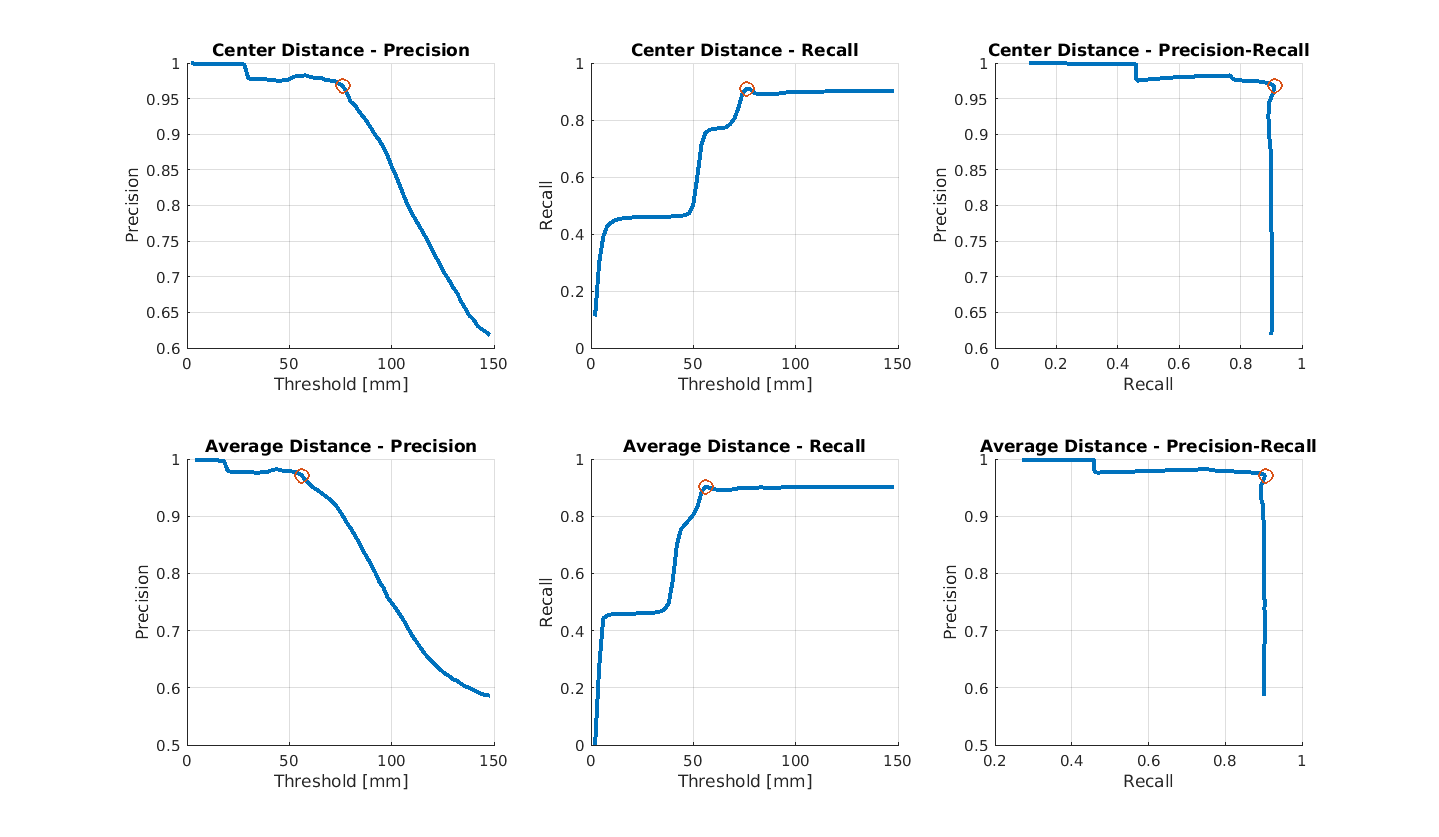
\includegraphics[width=\textwidth]{precision-recall.png}
    \caption{Precision and recall for both distance metrics on the button dataset. The point with the best F1 score is highlighted by a red circle.}
    \label{fig:precisionrecall}
\end{figure}

As can be seen from the figure, higher thresholds greatly impact the precision of our model while lower thresholds greatly impact its recall. Overall we maintain high values, but our maximum recall is limited by the performance of the network to a maximum of abount 90\%. To select the optimal threshold, we consider the F1 score, which is a balanced function of precision and recall:

\begin{equation*}
    \text{F1} = 2\times\frac{\text{Precision}\times\text{Recall}}{\text{Precision}+\text{Recall}}
\end{equation*}

For the average symmetric distance method, this results in a maximum F1 score of 0.9369, corresponding to a threshold of 56 mm, while for the center-to-center method the maximum is 0.9255, corresponging to a 78 mm threshold. A few observations can be made with these results.

First of all, for our application there is no great advantage in using average distance over center-to-center. Given the additional complexity and computation time, the increase in performance is not significant.

Second is that we have an abnormally high threshold for both methods. This can be attributed to the generated dataset: by stating that the buttons can only be either inside a slot or placed on the surface, we are in fact considering an ideal situation where a hypothetical manipulator does not commit any errors in picking up and inserting the buttons in their slots. If botched attempts are considered in the dataset, it is likely that the optimal threshold will be lower, and that the average distance method, being more adaptable to situations with different rotations, may give better results than center-to-center.

Finally, the threshold is also influenced by the probability distribution we used for generating the poses for the button dataset, which in our case being a uniform distribution resulted in a more spread-out placement, thus a higher optimal threshold. This is further compounded by the brute-force collision avoidance strategy implemented within the placement algorithm: if a placement attempt would generate an intersection with an already placed object, the placement was simply re-attempted from scratch. This naturally results in less conditions where dataset objects are in close proximity, and therefore in a higher threshold.

However it must be noted that creating a real-life dataset for determining the optimal threshold is much more approachable than creating a dataset for training a pose estimation network, as the ground truths are easy to aquire without any errors.